% ----------------------------------------------------------------
%% Thesis.tex -- MAIN FILE (the one that you compile with LaTeX)
%% ----------------------------------------------------------------

% Set up the document
\documentclass[a4paper, 11pt, twoside, openright]{Thesis}  % Use the "Thesis" style, based on the ECS Thesis style by Steve Gunn
\graphicspath{{res/Figures/}}  % Location of the graphics files (set up for graphics to be in PDF format)

% Include any extra LaTeX packages required
\usepackage[square, numbers, comma, sort&compress]{natbib}  % Use the "Natbib" style for the references in the Bibliography
\usepackage{verbatim}  % Needed for the "comment" environment to make LaTeX comments
\usepackage{vector}  % Allows "\bvec{}" and "\buvec{}" for "blackboard" style bold vectors in maths
\usepackage{algorithm}
\usepackage{algorithmic}
\usepackage[T1]{fontenc}

\usepackage{subcaption}
\usepackage{venturis2}
\usepackage{lmodern}
\usepackage{textcomp}    % solve issues with lmodern
\usepackage{amsfonts}
\usepackage{amsmath}
\usepackage{amsthm}
\usepackage{mathrsfs}
\usepackage{amssymb}
\usepackage{microtype}   % better typesetting with pdfLaTeX
\usepackage{ps4pdf}

\usepackage{verbatim}
\usepackage{algorithm}
\usepackage{algorithmic}
\usepackage{graphicx}
\usepackage{caption}
\usepackage{mathtools}
\usepackage{color}

\usepackage{booktabs}
\usepackage{multirow}
\usepackage{blindtext}

\usepackage{csvsimple}

\title{\LaTeX}

\date{}

\newtheorem{mydef}{Definition}
\newtheorem{myex}{Example}
\newtheorem{myprob}{Problem}
\PSforPDF{
  \usepackage{pstricks}
}
\usepackage[compact]{titlesec}
\usepackage{booktabs}
\usepackage{sectsty}     % section titles in specified font face
%\usepackage{listings}
\usepackage{listingsutf8}
\usepackage{caption}
\usepackage{xcolor}

\usepackage{enumitem}
\newcommand\litem[1]{\item{\bfseries #1}} % for labeled items (see tools used)

\allsectionsfont{\sffamily}
\numberwithin{algorithm}{chapter}
\setcounter{secnumdepth}{3}
\setcounter{tocdepth}{2}
\renewcommand{\captionlabelfont}{\sffamily\bfseries}
\newtheorem{thm}{Theorem}
\renewcommand{\algorithmicrequire}{\textbf{Input:}}
\renewcommand{\algorithmicensure}{\textbf{Output:}}
\newcommand{\term}[1]{{\sf {\small #1}}}
\hypersetup{urlcolor=black, colorlinks=false}  % Colours hyperlinks in blue, but this can be distracting if there are many links.

%global
\newcommand{\codedir}[0]{res/code}
\newcommand{\exampledir}[0]{codeexample}

% Chapter1:
\newcommand{\somecfile}{\codedir/\exampledir/rsa_crpt.c}

\newcommand{\interestingstart}{82}
\newcommand{\interestingend}{108}


% ---- TODO ----
\newcommand{\TODO}[1]{
	\textcolor{red}{#1}
}
\newcommand{\notsure}[1]{
	\textcolor{blue}{#1}
}
\usepackage{tikz}
\usetikzlibrary{automata, arrows.meta, positioning}
\usetikzlibrary{shapes.geometric, arrows}

\listfiles

%\usepackage[draft]{hyperref}
%\usepackage[hyperfootnotes=false,plainpages=false]{hyperref}
%% ----------------------------------------------------------------
\begin{document}
\frontmatter	  % Begin Roman style (i, ii, iii, iv...) page numbering

% Set up the Title Page
\title  {Link Stealing Attacks on Inductive Trained Graph Neural Networks}
\authors  {Philipp Zimmermann}
\addresses  {\groupname\\\deptname\\\univname}  % Do not change this here, instead these must be set in the "Thesis.cls" file, please look through it instead
\UNIVERSITY {\texorpdfstring{\href{https://www.uni-saarland.de}
            {Universit\"at des Saarlandes}}
            {Universit\"at des Saarlandes}}
\faculty{MI Fakult\"at f\"ur Mathematik und Informatik}
\department{\texorpdfstring{\href{https://saarland-informatics-campus.de/}
            {Department of Computer Science}}
            {Department of Computer Science}}
\reviewers{Dr. Yang Zhang}{.}
\date       {\today}
\subject    {}
\keywords   {}
\thesistype {Bachelorthesis}
\handin     {September 14, 2021}
\ifdefined\texhash
    \version {\texhash}
\else
    \version{}
\fi
\maketitle
%% ----------------------------------------------------------------

\setstretch{1.3}  % It is better to have smaller font and larger line spacing than the other way round

% Define the page headers using the FancyHdr package and set up for one-sided printing
%\fancyhead{}  % Clears all page headers and footers
%\rhead{\thepage}  % Sets the right side header to show the page number
%\lhead{}  % Clears the left side page header

\pagestyle{fancy}  % Finally, use the "fancy" page style to implement the FancyHdr headers
\fancyhead[RE,LO]{\sffamily\bfseries\nouppercase{\rightmark}}
\fancyhead[LE,RO]{\thepage}
%% ----------------------------------------------------------------
% Declaration Page required for the Thesis, your institution may give you a different text to place here
\vspace*{1cm}
\textbf{\large Eidesstattliche Erkl\"arung}\\[1em]
Ich erkl\"are hiermit an Eides statt, dass ich die vorliegende Arbeit selbst\"andig verfasst 
und keine anderen als die angegebenen Quellen und Hilfsmittel verwendet habe. 
\\[0.3cm]

\textbf{\large Statement in Lieu of an Oath}\\[1em]
I hereby confirm that I have written this thesis on my own and that I have not used any other media or materials than the ones referred to in this thesis.

Saarbr\"ucken, \handindate,\\[1.5cm]
\hspace*{1cm}(\authornames)\\[2cm]

\textbf{\large Einverst\"andniserkl\"arung}\\[1em]
Ich bin damit einverstanden, dass meine (bestandene) Arbeit in beiden Versionen in die Bibliothek der Informatik aufgenommen und damit ver\"offentlicht wird.
\\[0.3cm]

\textbf{\large Declaration of Consent}\\[1em]
I agree to make both versions of my thesis (with a passing grade) accessible to the public by having them added to the library of the Computer Science Department.

Saarbr\"ucken, \handindate,\\[1.5cm]
\hspace*{1cm}(\authornames)
\cleardoublepage

% END OF frontmatter.tex

%% ----------------------------------------------------------------
% The "Dedication Page"
%\pagestyle{empty}  % No headers or footers for the following pages

%\null\vfill\vfill\vfill\vfill\vfill
% Now comes the "Dedication Page", written in italics

Yes, you can

\vfill\vfill\vfill\vfill\vfill\vfill\null
\cleardoublepage  % Dedication page ended, start a new page


%% ----------------------------------------------------------------
\pagestyle{empty}


\begin{abstract}
	\justifying \noindent
	
	
	% Machine Learning experienced incredible boom in last decades \par
	% Big Data leads to huge amount of data available for training ML models \par
	% Graph Neural Networks operate on Graphs that can represent huge amount of data \par
	% In most cases sensitive / private ( Social Networks, Medical Data ) \par 
	% Neural Networks have been extended by processing / learning on graphs \par

\end{abstract}
%% ----------------------------------------------------------------
\pagestyle{empty}
\mbox{}
\clearpage
\setstretch{1.3}  % Reset the line-spacing to 1.3 for body text (if it has changed)

% The Acknowledgments page, for thanking everyone
\acknowledgements{
\addtocontents{toc}{\vspace{1em}}  % Add a gap in the Contents, for aesthetics



}
\clearpage
% End of the Acknowledgments

%% ----------------------------------------------------------------

\pagestyle{fancy}  %The page style headers have been "empty" all this time, now use the "fancy" headers as defined before to bring them back



%% ----------------------------------------------------------------
%\lhead{\emph{Contents}}  % Set the left side page header to "Contents"
\tableofcontents  % Write out the Table of Contents

%% ----------------------------------------------------------------
\setstretch{1.5}  % Set the line spacing to 1.5, this makes the following tables easier to read
\clearpage  % Start a new page
%\lhead{\emph{Abbreviations}}  % Set the left side page header to "Abbreviations"
%\listofsymbols{ll}  % Include a list of Abbreviations (a table of two columns)
%{
% \textbf{Acronym} & \textbf{W}hat (it) \textbf{S}tands \textbf{F}or \\
%\textbf{LAH} & \textbf{L}ist \textbf{A}bbreviations \textbf{H}ere \\

%}

%% ----------------------------------------------------------------
%\clearpage  %Start a new page
%\lhead{\emph{Symbols}}  % Set the left side page header to "Symbols"
%\listofnomenclature{lll}  % Include a list of Symbols (a three column table)
%{
% symbol & name & unit \\
%$a$ & distance & m \\
%$P$ & power & W (Js$^{-1}$) \\
%& & \\ % Gap to separate the Roman symbols from the Greek
%$\omega$ & angular frequency & rads$^{-1}$ \\
%}
%% ----------------------------------------------------------------
% End of the pre-able, contents and lists of things
% Begin the Dedication page

\setstretch{1.3}  % Return the line spacing back to 1.3

%\pagestyle{empty}  % Page style needs to be empty for this page

\addtocontents{toc}{\vspace{2em}}  % Add a gap in the Contents, for aesthetics


%% ----------------------------------------------------------------
\mainmatter	  % Begin normal, numeric (1,2,3...) page numbering
\pagestyle{fancy}  % Return the page headers back to the "fancy" style

% Include the chapters of the thesis, as separate files
% Just uncomment the lines as you write the chapters




%%%%%%%%%%%%%%%%%%%%%%%%%%%%%%%%%%%%%%%%%%%%%%%%%%%%%%%%%%%%%%%%%%%%%%%%%%%%%%%%%%%%%%%%%%%%%%%%%%%%%%%%%%%%%%%%%%%%%%%%%%%%%%%%%

\chapter{Introduction}

	% Figure Example
	% \begin{figure}
		% 	\lstinputlisting[language=C, firstline=\interestingstart, lastline=\interestingend]{\somecfile}
		% 	\caption{caption}
		% 	\label{code:aes_unsealdata}
		% \end{figure}

	\section{Motivation}
		A graph is a datastructure which is used to model large data and the relationships between entities.
		It consists of nodes and edges and can be used to model data in almost every domain.
		For example in social networks, healthcare analytics or protein-protein interactions.
		In a social network, the nodes would be the users that are registered and the edges would represent whether the users know each other or not by connecting them or not.
		A graph itself can be deemed as intellectual property of the data owner, since she may spent lots of time and resources collecting and preparing the data.
		In most cases the graph is also highly confidential because it contains sensitive information like private social relationships between users in a social network or medical information about specific people in healthcare-analytic datasets.
		Since nowadays graphs are a common way to store and visualize data, Machine Learning algorithms have been improved to directly operate on them.
		These Machine Learning Models are called Graph Neural Networks.
		



	\section{Outline}
		\TODO{write at the end}

Some citation\cite{Anderson:1972}
 % Introduction

\chapter{Related Work}

  % First Attacks
  Ever since machine learning algorithms were developed, there have been new attacks against these models.
  In 2004, Dalvi et al. proposed simple evasion attacks to defeat linear classifiers that are used in spam filters \cite{10.1145/1014052.1014066}.
  Later in 2006, Barreno et al. outline a broad taxonomy of attacks against linear classifier in their paper \emph{Can Machine Learning Be Secure?}\cite{10.1145/1128817.1128824}.
  After Deep Neural Networks began to dominate different domains in year 2012, attacks against these models were also found and further developed \cite{szegedy2014intriguing, Biggio_2018}.
  Today it is well known, that Machine Learning Models are vulnerable in a security and privacy manner and that there exist many attacks against Machine Learning Models.
  % Membership Inference
  With \emph{Membership Inference Attacks} \cite{carlini2019secret, chen2018differentially, 7958568, truex2019demystifying, hayes2018logan} an adversary aims to distinguish whether a given data sample was part of the training dataset of the target model or not.
  Shokri et al. \cite{7958568} proposed the first Membership Inference Attack on Machine Learning Models.
  Given a data record and black-box access to a model, they were able to determine if the record was in the target models training dataset.
  The authors used adversarial machine learning to train an adversary model, that recognizes differences in the target models prediction.
  They evaluated their experiments on realistic datasets like a hospital discharge, whose membership is sensitive from the privacy perspective and showed that these models can be vulnerable to membership inference attacks. To prevent this attacks, many defenses have been proposed \cite{10.1145/3319535.3363201, 7958568, salem2018mlleaks, Li_2021}.
  % Model Inversion
  With \emph{Model Inversion Attacks} \cite{PMID:27077138, 8476925, 10.1145/2810103.2813677, chen2020improved}, an adversary aims to learn sensitive attributes of the target models training dataset.
  The first model inversion attack has been proposed by Fredrikson et al. \cite{PMID:27077138}.
  They showed, that given the target model and some demographic information about a patient, it is possible to predict the patient's genetic markers.
  The authors further investigated, that differential privacy mechanisms prevent their model inversion attacks, when the privacy budget is carefully selected.
  % Model Extraction
  With \emph{Model Extraction Attacks} \cite{atli2020extraction, juuti2019prada, tramer2016stealing}, an adversary aims to steal the model internals and uses this information to gradually train a substitute model that immitates the behaviour of the target.
  Tramèr et al. \cite{tramer2016stealing} proposed simple model extraction attacks, which were able to steal target models with near-perfect fidality.
  A similar aproach was proposed by Wang and Gong \cite{8418595}, who were able to successfully steal the hyperparameters of target models.
  To mitigate these attacks, many defenses have been proposed \cite{juuti2019prada, hu2021model, 272262, mori2021bodame}.
  For Example Juuti et al. \cite{juuti2019prada}, showed that they were able to detect all prior model extraction attacks with no false positives by raising an alarm when the distribution of consecutive API queries deviates from benign behavior.
  Hu and Pang \cite{hu2021model} proposed an effective defense against model extraction attacks on Generative Adversarial Networks \cite{goodfellow2014generative}, considering a trade-off between the utility and security of GANs.

  % Adversarial Attacks on Graph Neural Networks
  Since many real world problems can be represented as graphs, it was urgent to develop machine learning algorithms to fully utilize graph data.
  Therefor, so called Graph Neural Networks have been developed and already used in various tasks \cite{4700287, atwood2016diffusionconvolutional, kipf2017semisupervised, velickovic2018graph}.
  Although, recent work shows, that Graph Neural Networks are vulnerable to adversarial attacks as well \cite{agbcvmtgs, 10.1145/3366423.3380149, Z_gner_2018, Z_gner_2018, jin2020adversarial}.
  More precisely, an adversary can decrease the targets accuracy by manipulating the graph structure or node features.
  For example, Sun et al. \cite{10.1145/3366423.3380149} proposed node injection poisoning attacks, where adversarial nodes are injected into existing graphs to reduce the performance of classifying existing nodes.
  Zügner et al. \cite{Z_gner_2018} showed that even with only a few pertubations the accuracy of node classification significantly drops, while focusing on training and testing phase.
  Wang et al. \cite{agbcvmtgs} focused on adversarial collective classification.
  They formulate their attack as a graph-based optimization problem, which produces the edges that an attacker needs to manipulate to achieve its attack goal and als propose several techniques to solve the optimization problem.
  Lastly Jin et al. \cite{jin2020adversarial} categorized existing attacks and defenses, and reviewed the corresponding state-of-the-art methods. They also have developed a repository with representative algorithms.
  Our work is different, since we focus on stealing links from Graph Neural Networks.

  % First Link Stealing Attacks on Graph Neural Networks
  In recent work, He et al. proposed the first attacks on Graph Neural Networks to obtain information about the underlaying training graph \cite{DBLP:journals/corr/abs-2005-02131}.
  They call their attacks \emph{Link Stealing Attacks}.
  Given black box access to a transductive trained Graph Neural Network, they showed that an adversary is able to predict whether any two nodes of a graph, that was used for training, are linked or not.
  The attacks reveal serious concerns on the intellectual property, confidentiality and privacy of graphs, when they are used for training.
  Our work is different, since we focus on \emph{Link Stealing Attacks} on inductive trained Graph Neural Networks.
  Specifically, given black box access to an inductive trained Graph Neural Network, we aim to predict whether there exists a link between any two nodes of a graph, that was used for training.
 % Related Work

\chapter{Background}

  \section{Neural Networks}

    Neural Networks (NNs) are key components in Artificial Intelligence (AI) and Deep Learning.
    They try to simulate some properties and the functionality of biological neural networks, like our brain, by imitating the way biological neural systems process data.
    Today, they have been applied successfully to speech recognition, face recognition on images or the transformation from speech to text.
    They are used to model software agents in video games, let autonomous robots learn new things or find patterns in data.

    A neural network consists of multiple layers.
    An input layer, one or many more hidden layers and an output layer.
    Each of these layers contain multiple neurons, which are represented as mathematical functions, that take multiple inputs and use them to calculate one output.
    Such neuron is also called perceptron, while fully connected neural networks are called multilayer perceptron (MLP).

    \vspace{0.48cm}
    \begin{figure}[!h]
      \begin{center}
        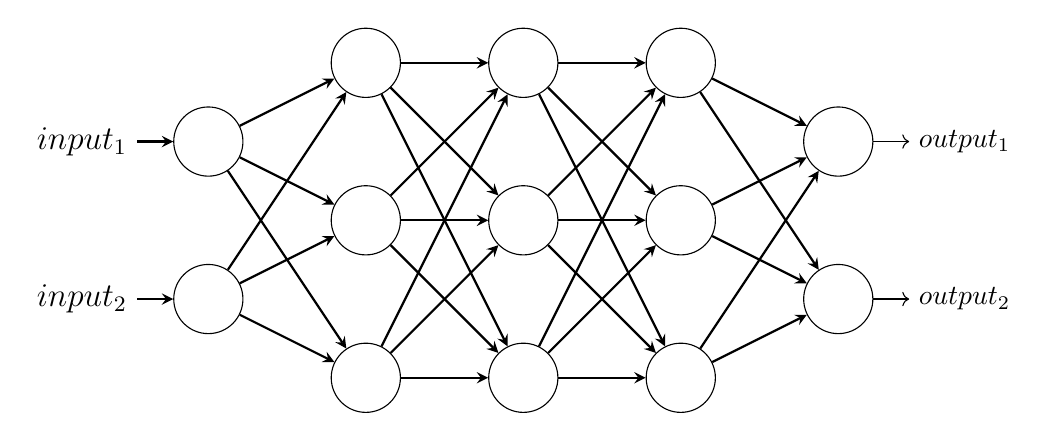
\begin{tikzpicture} [node distance = 2cm,
          on grid,
          %auto,
          %every state/.style = {draw = blue, fill = blue!30},
          every initial by arrow/.style = {font = \large,
              thick,-stealth
          }
          ]
          
          % Input Layer
          \node (i1) [state, initial, initial text= $input_1$] at (0,1) {};
          \node (i2) [state, initial, initial text= $input_2$] at (0,-1){};

          % Hidden Layer 1
          \node (h11) [state] at (2,2) {};
          \node (h12) [state] at (2,0) {};
          \node (h13) [state] at (2,-2) {};

          % Hidden Layer 2
          \node (h21) [state] at (4,2) {};
          \node (h22) [state] at (4,0) {};
          \node (h23) [state] at (4,-2) {};

          % Hidden Layer 2
          \node (h31) [state] at (6,2) {};
          \node (h32) [state] at (6,0) {};
          \node (h33) [state] at (6,-2) {};
          
          % Output Layer
          \node (o1) [state, accepting right, accepting text = {$output_1$}] at (8,1) {};
          \node (o2) [state, accepting right, accepting text = {$output_2$}] at (8,-1){};

          % Links
          \path [-stealth, thick]
            (i1) edge node {}   (h11)
            (i1) edge node {}   (h12)
            (i1) edge node {}   (h13)
            (i2) edge node {}   (h11)
            (i2) edge node {}   (h12)
            (i2) edge node {}   (h13)
            
            (h11) edge node {}   (h21)
            (h11) edge node {}   (h22)
            (h11) edge node {}   (h23)
            (h12) edge node {}   (h21)
            (h12) edge node {}   (h22)
            (h12) edge node {}   (h23)
            (h13) edge node {}   (h21)
            (h13) edge node {}   (h22)
            (h13) edge node {}   (h23)
            
            (h21) edge node {}   (h31)
            (h21) edge node {}   (h32)
            (h21) edge node {}   (h33)
            (h22) edge node {}   (h31)
            (h22) edge node {}   (h32)
            (h22) edge node {}   (h33)
            (h23) edge node {}   (h31)
            (h23) edge node {}   (h32)
            (h23) edge node {}   (h33)

            (h31) edge node {}   (o1)
            (h31) edge node {}   (o2)
            (h32) edge node {}   (o1)
            (h32) edge node {}   (o2)
            (h33) edge node {}   (o1)
            (h33) edge node {}   (o2);
        
        \end{tikzpicture}
      \end{center}

      \caption{Multilayer Perceptron}
      \label{figure:neural-network}
    \end{figure}

    \subsubsection*{Train a Neural Network}

      When we are confronted to a new task, we try to gain as much information as possible and based on them, we learn how to solve the problem.
      Neural networks behave similar.
      Before we can apply a neural network on classifying whether the object we provide is a spoon or fork, we need to tell the network, based on which information it should make its decision.
      That could be images of spoons and forks or their weight, length and width.
      We call this data \emph{Training Data}.
      To train the model in our example, we provide an image of a spoon and let the network make its decision.
      If the decision is correct, we wont change anything.
      But if the decision is incorrect, we need to slightly modify the weights - the connections between the perceptrons - to let the model behave different in the future.
      We do this for each image in our training set and repeat this process $n$ times (for $n$ epochs).
      After the training, we hopefully have a good trained neural network, which performs well on the provided task.

	\section{Graphs}

		As Graph we denote a data structure that contains nodes and edges. 
    Let $G = (V, E)$ be a graph with $V$ being the set of nodes and $E$ being the set of edges.
    We denote $\overrightarrow{a}$ as the feature vector of node $a$, representing the attributes of $a$.
    An edge $e = (i,j)$ contains the source node $i$ and the destination node $j$.
    In that way, links describe the relationship between the source and destination node. 
    The most popular example where graphs are used to model data, are social networks. 
    The nodes represent the users that have multiple attributes like location, gender, work place etc., while the edges state which relationship the users have.
    Lets consider a directed graph $G = (V,E)$ with $V$ representing the users and $E$ their relationships.
    If user $a$ follows user $b$, the edge $e_{ab} = (a,b)$ would be an element in $E$.
    If user $b$ follows user $a$, the edge $e_{ba} = (b,a)$ would be an element in $E$.
    Lets consider an undirected graph $G' = (V',E')$ with $V'$ representing the users and $E'$ their relationships.
    In $G'$ it doesn't matter whether user $a'$ follows $b'$ or the other way around. 
    Both results in $e'_{a'b'}, e'_{b'a'} \in E'$.
    Figure \refeq{figure:undirected-graph} shows an undirected graph.
    Since there is a link drawn between node $A$ and node $B$, we know, that there exists some relationship between them, but we don't know who follows whom ($e_{AB}, e_{BA} \in E$).
    The same holds for $e_{CF}, e_{FC} \in E$ or $e_{EG}, e_{GE} \in E$.
    Since there isn't a link drawn between node $E$ and node $C$, there doesn't exists a known relationship between them ($e_{EC}, e_{CE} \not\in E$).

    \vspace{0.48cm}
    \begin{figure}[!h]
      \begin{center}
        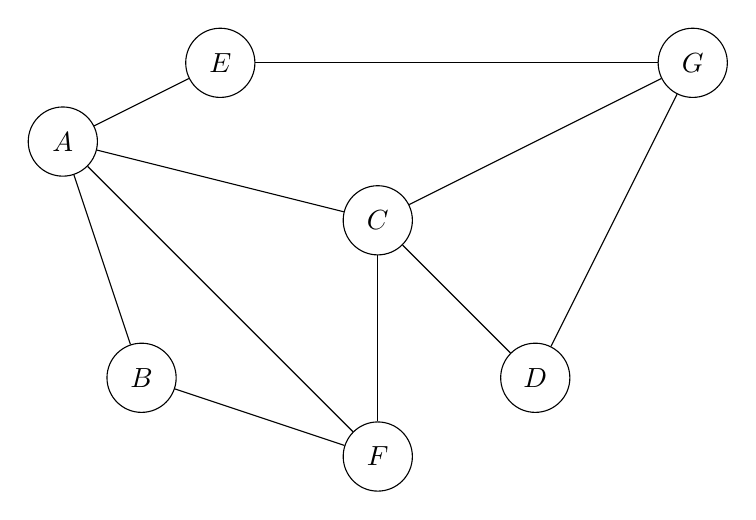
\begin{tikzpicture} [node distance = 2cm,
          on grid,
          %auto,
          %every state/.style = {draw = orange, fill = orange!30},
          every initial by arrow/.style = {font = \large,
              thick,-stealth
          }
          ]
          
          \node (a) [state] at (-1,2) {$A$};
          \node (b) [state] at (0,-1){$B$};
          \node (c) [state] at (3,1){$C$};
          \node (d) [state] at (5,-1){$D$};
          \node (e) [state] at (1,3){$E$};
          \node (f) [state] at (3,-2){$F$};
          \node (g) [state] at (7,3){$G$};

          % Links
          \draw (a) -- (b);
          \draw (d) -- (c);
          \draw (f) -- (a);
          \draw (a) -- (e);
          \draw (b) -- (f);
          \draw (c) -- (f);
          \draw (c) -- (g);
          \draw (d) -- (g);
          \draw (a) -- (c);
          \draw (e) -- (g);
        
        \end{tikzpicture}
      \end{center}

      \caption{Undirected Graph}
      \label{figure:undirected-graph}
    \end{figure}

	\section{Graph Neural Networks}
      
    % Describe how to query a graph neural network (f(Graph, node))
    In the last decades, social networks have become a huge part of life for many people all around the world.
    The companies behind these networks collect tons of data of each user every day.
    Let $G = (V, E)$ be a graph that models such a social network. 
    The set of all users is given as $V$ and $E$ represents their relationships.
    The feature vector $\overrightarrow{a}$ of user $a$ contains all information the company already has regarding this user.
    That could be name, relationship status, workplace, address, amount of children and so on.
    Lets consider one attribute (\emph{workplace}) as non mandatory for the registration.
    This leads to some users $v_{workplace} = \{v $ | $ \forall v \in V: v$ has $workplace$ given$\}$, the company knows the workplace from and some users $v_{unknown} = \{v $ | $ \forall v \in V: v$ has $workplace$ not given$\}$, where the attribute is unknown.
    Based on the information $v_{workplace}$ provides, a graph neural network model $f$ can be trained to predict the missing attribute of all users in $v_{unknown}$.
    This is a simple node classification task, where the label is the missing attribute $worplace$.
    There exist two major ideas of training a graph neural network - transductive or inductive.
    In our experiments introduced and described in Chapter \refeq{chapter:attacks} we focus on attacks on inductive trained graph neural networks. 

    \subsection*{Train a Graph Neural Network}

      To describe the process of training a graph neural network, we will stick to the example above.
      Let $f$ be the GNN we want to train on an undirected graph $G = (V,E)$ to perform some node classification task.
      We denote $workplace$ as label, that we want to predict and $V = v_{workplace} \cup v_{unknown}$ as set of nodes, containing every node, no matter whether the label is given or not.
      As our training dataset we define $d_{train} = \{(v, v_n)$ | $ \forall v \in v_{workplace}: v_n = neighborhood(v)\}$, where $neighborhood(n)$ is a function defined to collect the $k$-hop neighborhood of $n$ and aggregates their feature vectors. 
      $k = 0$ only considers $n$ and no neighbors of $n$.
      $k = 1$ also includes the neighbors of $n$, while $k = 2$ also aggregates the neighbors of the neighbors of $n$. 
      Depending on the type of GNN, this aggregation function $neighborhood()$ can differ in the algorithm collecting the neighborhood vectors.

      \subsubsection*{Transductive Learning}

        For transductive learning we consider all information as given, especially while training the graph neural network.
        More precisely, we denote, as mentioned before, $V = v_{workplace} \cup v_{unknown}$.
        This means, that for training the model on $d_{train}$, which contains all labeled nodes, the feature vectors of nodes, that are not labeled are included as well.
        Later when the model will be evaluated and tested, it already has seen the feature vectors of the nodes it should predict the labels of.
        So, the information of the nodes, the model needs to classify, is already known during the training phase.

      \subsubsection*{Inductive Learning}

        For inductive learning, we only consider the information of nodes that are labeled given while training the graph neural network.
        More precisely, we denote $V = v_{workplace}$ and $d_{train} = \{(v, v_n)$ | $ \forall v \in V: v_n = neighborhood(v)\}$.
        This means, that for training the model on $d_{train}$ only labeled nodes are used.
        Lets assume that three new users register to the social network, nobody setting his / her workplace.
        Since some other mandatory information and maybe some links are given, the graph neural network can be used to predict the workplace of the new users nevertheless they haven't been included in the training process.
        So, it is possible to train the graph neural network on some graph and apply it on others, since it is easy adjustable.
        
      Since the most real world problems like friendship prediction in social networks or protein-protein interactions in chemical networks cannot be modeled with a static graph, the inductive learning method is commonly used, while the transductive one isn't.
      In our work, we show that given an inductive trained graph neural network, that was trained on a graph $G_1$, we are able to extract information of another graph $G_2$ that is completely unknown to the model.
      More precisely, we steal links from $G_2$ using the prediction posteriors of the model while querying it on $G_2$.


 % Background

\chapter{Attacks}

  In recent work He et al. \cite{DBLP:journals/corr/abs-2005-02131} proposed the first link stealing attacks on graph neural networks.
  They focused on stealing links of the graph that was used for training the given target model.
  Like described in Section 3.3.1 this is an attack on transductive trained graph neural networks.
  In our work, we want to show, that it is possible for an attacker to steal links from graphs, given an inductive trained graph neural network.
  Therefor we assume the attacker has a graph, but is not sure about the completeness of the edges. Especially, maybe there are some edges between nodes missing in the graph.
  For two given nodes $i$ and $j$, we want to infer whether they are connected or not. More precisely, whether the edge is missing or really isn't existent in the attackers graph.
  To do so, we propose three attacks with two different thread models and two ways of training the attacker model.

  \section{Attack 1}

    In this section, we propose our first attack. Given a target graph neural network and a graph of the same dataset, that wasn't used for training the target model, an adversary aims to steal missing edges of its graph.
    Therefor it uses the posterior output of the two nodes, it queries the network on and concatenates them to get the feature, the attacker is then trained on.

    \subsection{Thread Model}

      In this attack the adversary has \emph{Black-Box Access} (Query-Access) to the target model and uses a subgraph of the same dataset distribution, the target model also was trained on.
      However, the adversary's graph wasn't used for training the target model.

    \subsection{Attack Methodology}

      To perform this attack, we split one of our used datasets, which will be covered in Section \TODO{update section}, into one traingraph and one testgraph. Given our dataset $G = (V, E)$ we calculate the traingraph  $G\textsubscript{train} = (V\textsubscript{train}, E\textsubscript{train})$ and the testgraph
      $G\textsubscript{test} = (V\textsubscript{test}, E\textsubscript{test})$ in the following way. $V\textsubscript{train} = \{i | \forall i \in V: random(0, 1) == 1\}$, where $random(0, 1)$ returns the values $0$ or $1$ at random, leading to a random split of the nodes.
      $E\textsubscript{train} = \{(i, j) | \forall (i,j) \in E: i, j \in V\textsubscript{train}\}$ now contains the edge $(i,j)$ if both nodes $i$ and $j$ are in $V\textsubscript{train}$.
      The testgraph is now calculated similary.
      $V\textsubscript{test} = \{j | \forall j \in V: j \not\in V\textsubscript{train}\}$ and $E\textsubscript{test} = \{(i, j) | \forall (i,j) \in E: i, j \in V\textsubscript{test}\}$

      \subsubsection{Target Model}

        The target model is now trained on $G\textsubscript{train}$ to perform node classification.
        Especially, given a node's features, its neighbors' and the edges between them, the model outputs a prediction posterior of the class.

      \subsubsection{Attacker Model}

        We first create a raw dataset \emph{da-raw} for the attacker model based on $G\textsubscript{test}$ of our dataset.
        To do so, we create a clone of the testgraph $G\textsubscript{adv} = G\textsubscript{test}$, which will represent the adversary's graph.
        We now collect a set of positive samples $pos = \{(i,j, 1) | \forall i,j \in V\textsubscript{test}: (i,j) \in E\textsubscript{test} \wedge |pos| < ((1 - \alpha) * |E\textsubscript{test}|))\}$, containing pairs of nodes, that are connected in the testgraph, where $\alpha$ denotes the percentage of known edges.
        We then delete all edges we sampled, in our graph clone $E\textsubscript{adv} = \{(i,j) | \forall (i,j) \in E\textsubscript{adv}: (i,j) \not\in pos\}$, to represent the missing edges, we want to steal.
        Now, we collect a set of negative samples $neg = \{(i,j, 0) | \forall i,j \in V\textsubscript{test}: (i,j) \not\in E\textsubscript{test} \wedge |neg| < ((1 - \alpha) * |E\textsubscript{test}|))\}$, containing pairs of nodes, that are not connected in $G\textsubscript{test}$.
        Our raw dataset \emph{da-raw} = $pos \cup neg$, now contains positive and negative samples obtained from $G\textsubscript{test}$.
        As the next step, we create the adversary's dataset $da = \{(post_i_j, l) | \forall (i,j,l)\in\emph{da-raw}: post_i_j = concat(target(G\textsubscript{adv}, i), target(G\textsubscript{adv}, j))\}$.
        $target(G\textsubscript{adv}, i)$ returns the node classification output posterior of the target model, when it is queried on $i$ given the adversary's graph $G\textsubscript{adv}$.
        $concat(a, b)$ concatenates the output posteriors $a$ and $b$ with each other returning the feature we will train the attacker model on.
        $l$ denotes the label either being 1 (positive sample) or 0 (negative sample).
        With our adversary's dataset $da$ we can now continue training our attacker model using $post_i_j$ as input features and $l$ as class.

  \section{Attack 2}

    In this section, we propose our second attack. Given a target graph neural network and a graph of the same dataset, that wasn't used for training the target model, an adversary aims to steal missing edges of its graph.
    Therefor it uses the posterior output of the two nodes, it queries the network on and calculates the distance between these two vectors in eight different ways and uses these values as input features for training the attacker model.

    \subsection{Thread Model}

      The Thread Model for this attack is the same one described in Section 4.1.1.

    \subsection{Attack Methodology}

      Most of the Attack Methodology is the same as the one described in Section 4.1.2.
      There is one difference however.
      Instead of using the concatenation of the two output posteriors, we now use them as vectors, to calculate their distances in eight different ways.
      We have in total experimented with 8 common distance metrics: Cosine distance, Euclidean distance, Correlation distance, Chebyshev distance, Braycurtis distance, Canberra distance, Manhattan distance, and Square-euclidean distance.

      \subsubsection{Attacker}

        We first create \emph{da-raw} like described in Section 4.1.2.2.
        Our adversary's dataset can now be desribed as the following.
        $da = \{(dist_i_j, l) | \forall (i,j,l)\in\emph{da-raw}: dist_i_j = d(target(G\textsubscript{adv}, i), target(G\textsubscript{adv}, j))\}$, where $d(a,b) = concat(dist_1(a,b), ..., dist_8(a,b))$ and $l$ again denotes the label.
        With our adversary's dataset $da$ we can now continue training our attacker model using $dist_i_j$ as input features and $l$ as class.

  \section{Attack 3}

    In this section, we propose our last attack. Given a target graph neural network and a graph of a different dataset, that wasn't used for training the target model, an adversary aims to steal missing edges of its graph.
    Therefor it uses the posterior output of the two nodes, it queries the network on and calculates the distance between these two vectors in eight different ways and uses these values as input features for training the attacker model.

    \subsection{Thread Model}

      In this attack the adversary has \emph{Black-Box Access} (Query-Access) to the target model and uses a different source dataset than the target.

    \subsection{Attack Methodology}

      As mentioned before, we now have two different datasets $G\textsubscript{target} = (V\textsubscript{target}, E\textsubscript{target})$ and $G\textsubscript{attacker\_model} = (V\textsubscript{attacker\_model}, E\textsubscript{attacker\_model})$.

      \subsubsection{Target}

        The target model is now trained on $G\textsubscript{target}$ to perform node classification.
        Especially,given a node’s features, its neighbors’ and the edges between them, the model outputs aprediction posterior of the class.

      \subsubsection{Attacker Model}

        We first create the raw dataset \emph{da-raw} the same way, we did before but this time with $G\textsubscript{attacker\_model}$.
        To do so, we again create a clone $G\textsubscript{adv} = G\textsubscript{attacker\_model}$.
        We now collect a set of positive samples $pos = \{(i,j, 1) | \forall i,j \in V\textsubscript{attacker\_model}: (i,j) \in E\textsubscript{attacker\_model} \wedge |pos| < ((1 - \alpha) * |E\textsubscript{attacker\_model}|))\}$.
        We then delete all edges we sampled, in our graph clone $E\textsubscript{attacker\_model} = \{(i,j) | \forall (i,j) \in E\textsubscript{adv}: (i,j) \not\in pos\}$, to represent the missing edges, we want to steal.
        Now, we collect a set of negative samples $neg = \{(i,j, 0) | \forall i,j \in V\textsubscript{attacker\_model}: (i,j) \not\in E\textsubscript{test} \wedge |neg| < ((1 - \alpha) * |E\textsubscript{attacker\_model}|))\}$, containing pairs of nodes, that are not connected in $G\textsubscript{attacker\_model}$.
        Our raw dataset \emph{da-raw} = $pos \cup neg$, now contains positive and negative samples obtained from $G\textsubscript{attacker\_model}$.
        As the next step, we create the adversary's dataset $da = \{(dist_i_j, l) | \forall (i,j,l)\in\emph{da-raw}: dist_i_j = d(target(G\textsubscript{adv}, i), target(G\textsubscript{adv}, j))\}$, where $d(a,b) = concat(dist_1(a,b), ..., dist_8(a,b))$ and $l$ again denotes the label.
        With our adversary's dataset $da$ we can now continue training our attacker model using $dist_i_j$ as input features and $l$ as class.
 % Attacks

\chapter{Implementation}

  In order to analyze how effective our attacks can steal links from the training graph of an inductive trained graph neural network, we performed several experiments by attacking GNNs that have been trained to perform node classification.
  In this chapter we want to go through the implementation of our attacks.
  We covered multiple datasets and types of graph neural network models, leading to an amount of \textasciitilde200 experiments.
  Due computational and time constraints, most of the parameters to optimize the attacks remain unexplored.

  \section{Datasets}
  \label{section:datasets}

    For all our experiments, we used 3 datasets in total.
    In the table below, they are listed with their most interesting attributes.
    All of the datasets we used are from the same domain - Citation Networks.
    This is because these networks are open source and similar to social networks in their structure.
    Due to computational constraints we didn't use social network datasets like reddit.

    \vspace{0.48cm}
    \begin{table}[!h]
      \centering
      \footnotesize
      \begin{tabular}{l|l|l|l|l}
        \toprule
        Name & Number of Nodes & Number of Edges & Number of Classes & Feature Amount \\
        \midrule
        Cora & 2708            & 5429            & 7                 & 1433 \\
        CiteSeer & 3327        & 4732            & 6                 & 3703 \\
        Pubmed & 19717         & 44338           & 3                 & 500 \\
        \bottomrule
      \end{tabular}
      \caption{Dataset Information}
      \label{table:datasets}
    \end{table}

    \subsection*{Sample Datasets for Experiments}
    \label{subsection:dataset-samples}

      In total we train target models on all three datasets - \emph{Cora}, \emph{CiteSeer} and \emph{Pubmed} .
      To train the attacker models, we sample an adversary dataset based on the incomplete subgraph.

      \subsubsection*{Same Dataset Distributions - Attack 1-2}
        Let $D_{f_t} = (V_{f_t}, E_{f_t})$ be one of our three original datasets with $|V_{f_t}|$ nodes and $|E_{f_t}|$ edges.
        We denote $D' = (V',E')$ as subgraph of $D_{f_t}$.
        $D_{f_t}$ is used to train our target model $f_t$, while $D'$ is used to sample $G_{A}$, which is a graph, that was modified by deleting some known edges to simulate an incomplete graph.
        $D_A$ is obtained by querying $f_t$ on a subgraph of $G_A$. 

        \vspace{0.48cm}
        \begin{figure}[h!]
          \begin{center}
            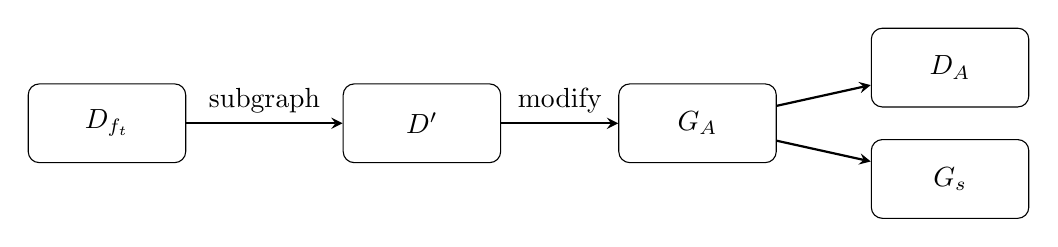
\begin{tikzpicture}
              
              % Definitions
              \tikzstyle{Dataset} = [rectangle, rounded corners,minimum width=2cm, minimum height=1cm, text centered, draw=black]
              \tikzstyle{arrow} = [thick,->,>=stealth]

              \node (Dft) [Dataset] {$D_{f_t}$};
              \node (D') [Dataset, right of=Dft, xshift=3cm] {$D'$};
              \node (GA) [Dataset, right of=D', xshift=2.5cm] {$G_A$};
              \node (DA) [Dataset, above right of=GA, xshift=2.5cm] {$D_A$};
              \node (Gs) [Dataset, below right of=GA, xshift=2.5cm] {$G_s$};

              \draw [arrow] (Dft) -- node[anchor=south] {subgraph} (D');
              \draw [arrow] (D') -- node[anchor=south] {modify} (GA);
              \draw [arrow] (GA) -- node[anchor=south] {} (Gs);
              \draw [arrow] (GA) -- node[anchor=south] {} (DA);

              

            \end{tikzpicture}
          \end{center}
          \caption{Sampling Datasets - Same Dataset Distribution - Attack 1-2}
          \label{figure:sample-datasets-attack1-2}
        \end{figure}

        We define $G_A = (V_A, E_A)$ with $V_A = V'$ and $E_A = E'$, which is now an exact copy of $D'$.
        To sample $D_A$, we first collect a set of positive samples $pos = \{(i,j, 1)$ | $\forall i,j \in V': (i,j) \in E' \wedge |pos| < ((1 - \alpha) * |E'|))\}$, containing pairs of nodes, that are connected in $D'$, where $\alpha$ denotes the percentage of known edges.
        Now, we collect a set of negative samples $neg = \{(i,j, 0)$ | $\forall i,j \in V': (i,j) \not\in E' \wedge |neg| < ((1 - \alpha) * |E'|))\}$, containing pairs of nodes, that are not connected in $D'$.
        We then delete all edges we sampled for $pos$, in our graph clone $G_A$, to simulate the missing edges, we want to steal.
        This leads to $E_A = \{(i,j)$ | $\forall (i,j) \in E': (i,j) \not\in pos\}$.
        $G_A$ is now a modified graph that contains less edges then the original graph $D'$ and we define a raw-dataset $raw = pos \cup neg$, containing the positive and negative samples obtained from $D'$.
        As the next step, we create the adversary's dataset $D_A = \{(post_{ij}, l)$ | $\forall (i,j,l)\in raw: post_{ij} = concat(f_t(G_A, i), f_t(G_A, j))\}$ for \emph{Attack 1} and $D_A = \{(dist_{ij}, l)$ | $\forall (i,j,l)\in raw: dist_{ij} = dist(post_i, post_j)\}$ for \emph{Attack 2}.
        $f_t(G_A, i)$ returns the node classification output posterior of the target model, when it is queried on $i$ given the adversary's graph $G_A$.
        $concat(a, b)$ concatenates the output posteriors $a$ and $b$ with each other returning the feature we will train the attacker model on.
        $l$ denotes the label either being 1 (positive sample) or 0 (negative sample).
        $dist(a,b) = [Cosine(a,b), ..., Sqeuclidean(a,b)]$, return the vector containing 8 different distance values like described in Section \refeq{section:threat-model}.
        With our adversary's dataset $D_A$ we can now continue training our attacker model using either $post_{ij}$ or $dist_{ij}$ as input features and $l$ as class.
        $G_s$ represents the incomplete subgraph of $D_{f_t}$, which will be used to test the adversary performance on $f_f$.
        More precisely, how well does the adversary can predict correctly whether a link between two nodes in $G_s$ is missing or not.

      \subsubsection*{Different Dataset Distributions - Attack 3}

        Let $D_{f_A}$ and $D_{f_t}$ be two of our three original datasets.
        We use $D_{f_A}$ to train the shadow model $f_A$ and $D_{f_t}$ to train our target model $f_t$.
        We denote $D_1'$ as subgraph of $D_{f_A}$ and $D_2'$ as subgraph of $D_{f_t}$.
        To sample $D_A$ we follow the same steps as described in \emph{Attack 1}.
        Firstly we create an incomplete graph $G_A$ by randomly deleting some edges.
        We then sample $D_A$ by querying $f_A$ on $G_A$.
        To obtain $G_s$ we modify $D_2'$ by randomly deleting some edges and use it to test the adversary performance on $f_t$.

        \vspace{0.48cm}
        \begin{figure}[h!]
          \begin{center}
            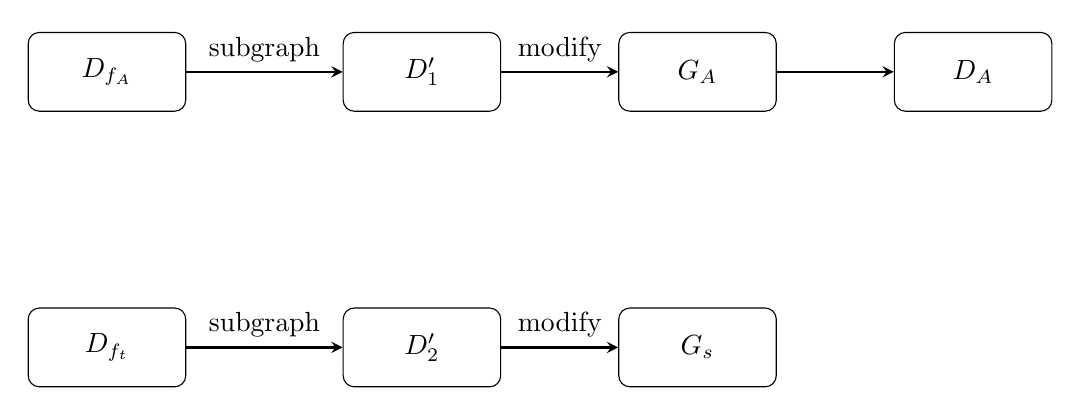
\begin{tikzpicture}
              
              % Definitions
              \tikzstyle{Dataset} = [rectangle, rounded corners,minimum width=2cm, minimum height=1cm, text centered, draw=black]
              \tikzstyle{arrow} = [thick,->,>=stealth]

              \node (Dfa) [Dataset] {$D_{f_A}$};
              \node (D1') [Dataset, right of= Dfa, xshift=3cm] {$D_1'$};
              \node (GA) [Dataset, right of= D1', xshift=2.5cm] {$G_A$};
              \node (DA) [Dataset, right of= GA, xshift=2.5cm] {$D_A$};


              \node (Dft) [Dataset, below of =Dfa, yshift=-2.5cm] {$D_{f_t}$};
              \node (D2') [Dataset, right of= Dft, xshift=3cm] {$D_2'$};
              \node (Gs) [Dataset, right of= D2', xshift=2.5cm] {$G_s$};
              
              \draw [arrow] (Dfa) -- node[anchor=south] {subgraph} (D1');
              \draw [arrow] (D1') -- node[anchor=south] {modify} (GA);
              \draw [arrow] (GA) -- node[anchor=south] {} (DA);

              \draw [arrow] (Dft) -- node[anchor=south] {subgraph} (D2');
              \draw [arrow] (D2') -- node[anchor=south] {modify} (Gs);
              

            \end{tikzpicture}
          \end{center}
          \caption{Sampling Datasets - Different Dataset Distribution - Attack 3}
          \label{figure:sample-datasets-attack3}
        \end{figure}

        However, this time the adversary was trained on another dataset distribution than the target model.
        E.g. the adversary was trained with the \emph{Cora} dataset.
        We then use $A$ to steal links from the training graph of a target model that was trained on the \emph{CiteSeer} dataset, considering an incomplete subgraph of the \emph{CiteSeer} dataset as $G_s$.
        Because of that we use $dist_{ij}$ as input for the attacker model instead of the posterior concatenation, like it was done in \emph{Attack 2}.


  \section{Target Models}

    As our target models, we used three different types of graph neural network models and trained them to perform a node classification task. 
    Therefor, we trained them on our three original datasets Cora, CiteSeer and Pubmed.

    \subsection*{GraphSAGE}
      In June 2017 Hamilton et al.\cite{hamilton2018inductive} proposed a general framework, called GraphSAGE (SAmple and aggreGatE), for inductive node embedding. 
      They came up with an idea of leveraging node features like text attributes, node profile information or node degrees to learn an embedding function that generalizes to unseen nodes instead of prior approaches that use matrix factorization.
      Until then, the training process focused on individual embeddings for each node, but with the GraphSAGE algorithm, a function is learned that generates embeddings by sampling and aggregating features from a node's neighborhood.

      Our graphsage target models are trained to perform a node classification task.
      In total we train three graphsage models - one for each dataset.
      The input layer contains as much neurons as the given datasets' samples provide features.
      Then, two hidden layers follow, each with 16 neurons.
      The number of output neurons is equal to the classes the dataset provides.
      We train each of them for 200 epochs with a learning rate of $0.01$ and dropout of $0.5$, achieving an average accuracy of $83\%$ for \emph{Cora}, $57\%$ for \emph{CiteSeer} and $89\%$ for \emph{Pubmed}.

    \subsection*{Graph Attention Networks}
      In October 2017 Velickovic et al.\cite{gat} presented graph attention networks (GATs), novel neural network architectures that operate directly on graphs.
      Without requiring any kind of matrix operation or knowledge about the local graph structure the authors specify different weights to different nodes in a nodes' neighborhood by stacking multiple layers in which nodes are able to attend over their neighborhoods' feature vectors.
      Based on this approach, GATs don't only address transductive but also inductive problems and have achieved or matched state-of-the-art results across four established transductive and inductive graph benchmarks.

      Our gat target models are trained to perform a node classification task.
      In total we train three gat models - one for each dataset.
      The input layer contains as much neurons as the given datasets' samples provide features.
      Then, one hidden layer with 8 neurons follows.
      The number of output neurons is equal to the classes the dataset provides.
      We train each of them for 200 epochs with a learning rate of $0.005$, dropout of $0.6$, achieving an average accuracy of $78\%$ for \emph{Cora}, $61\%$ for \emph{CiteSeer} and $89\%$ for \emph{Pubmed}.

    \subsection*{Graph Convolutional Networks}
      In February 2017 Kipf et al. \cite{gcn} proposed a scalable approach for semi-supervised learning on graph-structured data that is based on an efficient variant of convolutional neural networks which operate directly on graphs.
      Nevertheless, the authors only consider the transductive setting in their paper, the idea of the algorithm stays the same, when using it for inductive learning.
      To aggregate the neighborhood, the authors use a single weight matrix per layer and deal with varying node degrees through an appropriate normalization of the adjacency matrix.

      Our gcn target models are trained to perform a node classification task.
      In total we train three gcn models - one for each dataset.
      The input layer contains as much neurons as the given datasets' samples provide features.
      Then, two hidden layers follow, each with 16 neurons.
      The number of output neurons is equal to the classes the dataset provides.
      We train each of them for 200 epochs with a learning rate of $0.01$ and dropout of $0.5$, achieving an average accuracy of $76\%$ for \emph{Cora}, $57\%$ for \emph{CiteSeer} and $88\%$ for \emph{Pubmed}. 

    The following table provides an overview of our target models and their accuracies regarding their training datasets.
    Each of them has been trained for 200 epochs, a learning rate of $0.01$ (GraphSAGE and GCN) or $0.005$ (GAT) and a dropout of $0.5$ (GraphSAGE and GCN) or $0.6$ (GAT).
    \vspace{0.48cm}
    \begin{table}[!h]
      \centering
      \footnotesize
      \begin{tabular}{l|l|l|}
        \toprule
        Target Model & Dataset & Accuracy \\
        \midrule
          \multirow{3}{4em}{GraphSage} & Cora & $83\%$ \\
          & CiteSeer & $61\%$ \\
          & Pubmed & $89\%$ \\

          \multirow{3}{4em}{GAT} & Cora & $78\%$ \\
          & CiteSeer & $57\%$ \\
          & Pubmed & $89\%$ \\

          \multirow{3}{4em}{GCN} & Cora & $76\%$ \\
          & CiteSeer & $57\%$ \\
          & Pubmed & $88\%$ \\
          
        \bottomrule
      \end{tabular}
      \caption{Target Model Accuracies}
      \label{table:target-models}
    \end{table}

  \section{Attack Model}
    As our attack model we use a Multilayer Perceptron \refeq{figure:neural-network}.
    Depending on the attack, the MLP has eight (\emph{Attack 2} and \emph{Attack 3}) or two times the size of the posterior output of $f$ (\emph{Attack 1}) input neurons.
    Then two hidden layers with 16 neurons each follow.
    The final output layer consists of 2 neurons, representing the two cases of the two target nodes originally being connected or not.
    We trained our attack models on the obtained datasets $D_A$ for 200 epochs, with a learning rate of $0.01$ and dropout of $0.5$.
 % Implementation

\chapter{Evaluation}

    \section{Datasets}
        In total we used 3 different Datasets (Section \refeq{section:datasets}), which are common used benchmark datasets for evaluating Graph Neural Networks \cite{acharya2019feature, gao2019graphnas, gcn}.
        All of them are citation datasets with nodes being publications and edges representing citations among these publications.        
        Furthermore do all datasets contain nodes' attributes and labels.

        The method to sample the attack dataset $D_A$, described in Section \refeq{subsection:dataset-samples}, follows the common practice in the literature of link prediction \cite{BHPZ17, grover2016node2vec}.

    \section{Metric}
        We use F1-Score as our main evaluation metric.
        It is a common used metric in binary classification \cite{lipton2014thresholding, santus2016features, woodbridge2016predicting}, since it is the harmonic mean of precision and recall.-
        The highest value, that is possible, is 1.0, indicating perfect precision and recall.
        If either the precision or the recall is zero, the F1-Score is 0.0.
        Leading to f1-Score values between 0 and 1.

        \subsection*{Precision}
            A high precision represents a high probability that the prediction of a Machine Learning model is correct.
            Let $M$ be a Machine Learning model that was trained to predict whether an email is spam or not.
            High precision means, that when the model labels an email as malicious, it is correct most of the time and vice versa.

        \subsection*{Recall}
            A high recall represents a high percentage of correctly classified inputs.
            In the example just given, that means, that $M$ is able to identify a high amount of spam-mails as malicious.

    \section{Attack Performance}
        The results presented below are the average results of 10 runs.
        Meaning, that all attacks have been performed multiple times to get a better relation.
        Note, that the performance varies based on the random choice of the nodes that are included in the partial graph $G_s$.
        Each attack is performed on all target models, which have been trained on different datasets.
        As our baseline we consider that the partial graph $G_s$ doesn't contain any links.
        We then add 20\% of the edges per attack, ending up with 80\% known edges.

        \subsection*{Attack 1}
            Like described in Section \refeq{section:attack1} this attack performs link stealing attacks on the same dataset distribution using the concatenation of the posterior outputs of two nodes to infer whether they have been connected or not. 
            Figure \refeq{figure:eval-att1-citeseer} presents the results for our link stealing attacks on the target models, that have been trained on the CiteSeer dataset.
            Please find the results for Cora in Figure \refeq{figure:eval-att1-cora} and for Pubmed in Figure \refeq{figure:eval-att1-pubmed}

            \begin{figure}[h]
                \begin{center}
                    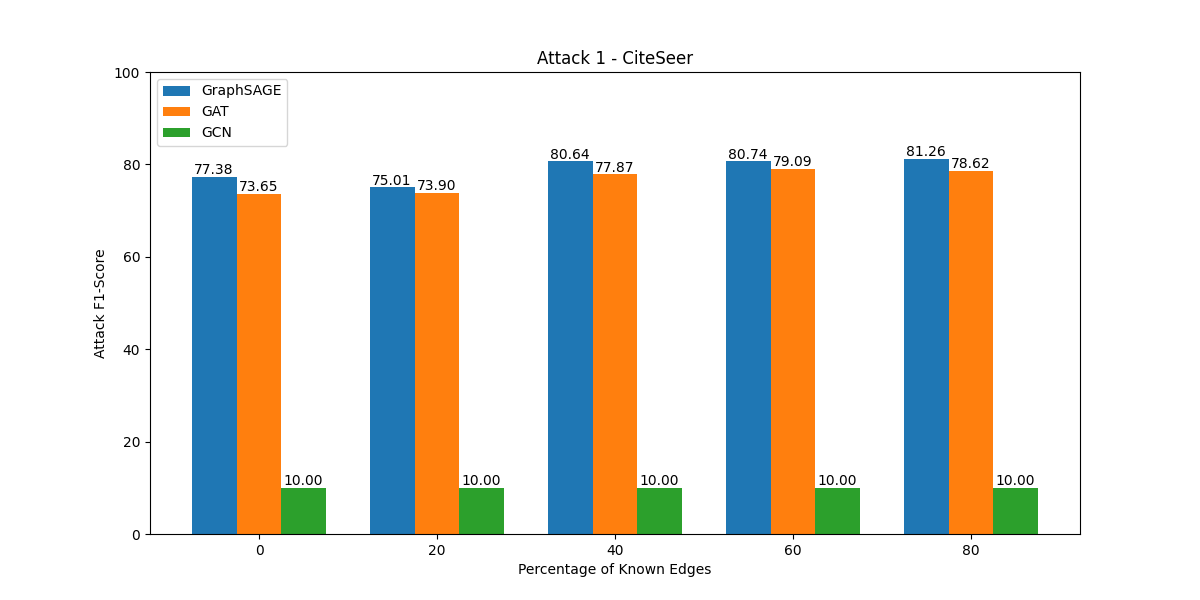
\includegraphics[width=\textwidth]{attack-1-citeseer}
                    \caption{Attack 1 - $D_{f_t} = CiteSeer$}
                    \label{figure:eval-att1-citeseer}
                \end{center}
            \end{figure}

            Note that our baseline already achieves an average F1-Score of $0.7421$ depending on Graph Neural Network type and target dataset $D_{f_t}$.
            The baseline performed best ($0.7903$ F1-Score) on the Graph Convolutional Neural Network, when it was trained on the  CiteSeer dataset and it performed worst ($0.6663$ F1-Score) on the Graph Attention Network when it was trained on the Cora dataset.
            Intuitively, with rising amount of known edges, we would expect a higher performance of our attacks.
            However, in some cases, the performance grows until 40\% or 60\% of known edges and drops afterwards.
            More precisely, sometimes the attack performance is better with only 60\% of known edges than with 80\%.
            The reason we observe this, is the following. 
            Since we use the deleted edges as positive samples for our training data, the more edges are known, the less data will be provided for training the attack model. 
            Leading to more training data in our baseline than in our 80\%-known-edges attack.
            With respect to all performed attacks, the average F1-Score is $0.7413$.
            Table \refeq{table:attack1-best-and-worst-performance} presents the F1-Scores of our best and worst attacks.

            \vspace{0.48cm}
            \begin{table}[!h]
                \centering
                \footnotesize
                \begin{tabular}{l|l|l|l|l|}
                \toprule
                Target Model & $D_{f_t}$ & $G_A$ Distribution & $\alpha$ & F1-Score \\
                \midrule
                GCN       & Cora   & Cora   & 0.8 & $0.8110$ \\
                GraphSAGE & Pubmed & Pubmed & 0.2 & $0.5643$ \\
                
                \bottomrule
                \end{tabular}
                \caption{Attack-1: Best and Worst Attack Performance}
                \label{table:attack1-best-and-worst-performance}
            \end{table}

        \subsection*{Attack 2}
            Like described in Section \refeq{section:attack2} this attack performs link stealing attacks on the same dataset distribution using the calculated distance vector of the posterior outputs of two nodes to infer whether they have been connected or not. 
            Figure \refeq{figure:eval-att2-citeseer} presents the results for our link stealing attacks on a target model, that was trained on the CiteSeer dataset.
            Please find the results for Cora in Figure \refeq{figure:eval-att2-cora} and for Pubmed in Figure \refeq{figure:eval-att2-pubmed}

            \begin{figure}[h]
                \begin{center}
                    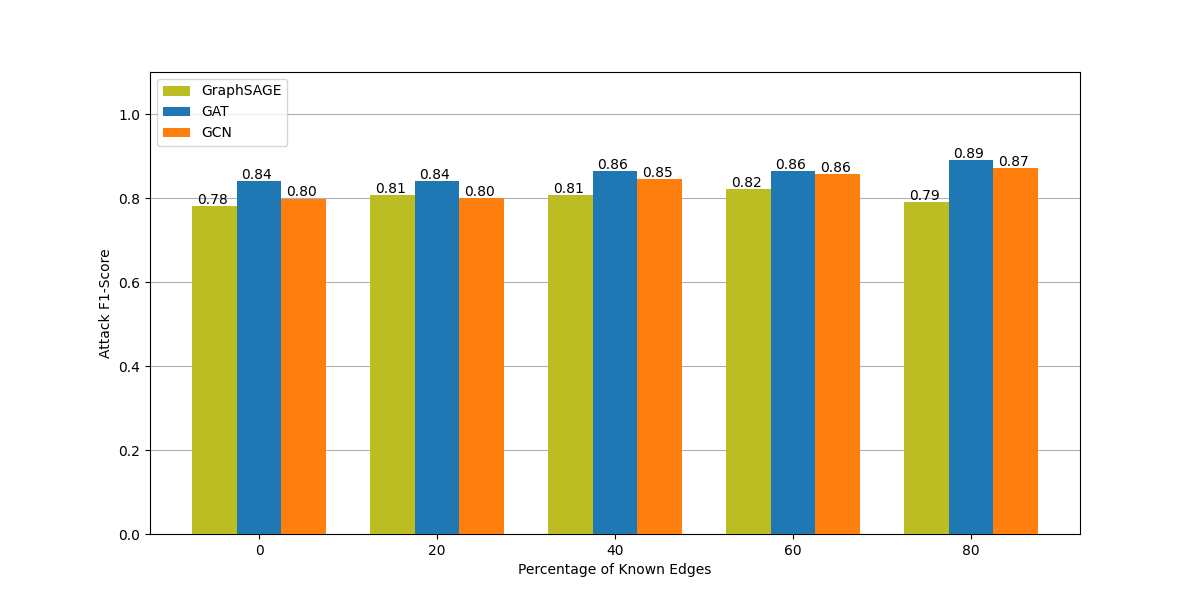
\includegraphics[width=\textwidth]{attack-2-citeseer}
                    \caption{Attack 2 - $D_{f_t} = CiteSeer$}
                    \label{figure:eval-att2-citeseer}
                \end{center}
            \end{figure}

            The first noticeable fact is, that using the distance vector instead of the concatenation of the posteriors is more effective.
            This time the average F1-Score of our baseline is $0.7770$, again depending on Graph Neural Network type and target dataset $D_{f_t}$.
            The baseline performed best ($0.8374$ F1-Score) on the Graph Attention Network, when it was trained on the CiteSeer dataset and it performed worst ($0.7535$ F1-Score) on the GraphSAGE GNN when it was trained on the Pubmed dataset.
            Again we can observe, that the results support our forecast.
            % calculate improvement: impr = max(20p, 40p, 60p, 80p) - baseline
            With rising amount of known edges, the attack performance grows, leading to an improvement up to $0.08$ F1-Score, while comparing the baseline performance with the results of attacks with more known edges.
            With respect to all performed attacks, the average F1-Score is $0.8049$.
            Table \refeq{table:attack2-best-and-worst-performance} presents the F1-Scores of our best and worst attacks.
            
            \vspace{0.48cm}
            \begin{table}[!h]
                \centering
                \footnotesize
                \begin{tabular}{l|l|l|l|l|}
                \toprule
                Target Model & $D_{f_t}$ & $G_A$ Distribution & $\alpha$ & F1-Score \\
                \midrule
                GAT       & CiteSeer & CiteSeer & 0.8 & $0.8923$ \\
                GraphSAGE & Cora     & Cora     & 0.8 & $0.7463$ \\
                
                \bottomrule
                \end{tabular}
                \caption{Attack-2: Best and Worst Attack Performance}
                \label{table:attack2-best-and-worst-performance}
            \end{table}

        \subsection*{Attack 3}
            Like described in Section \refeq{section:attack3} this attack performs link stealing attacks on a different dataset distribution using the calculated distance vector of the posterior outputs of two nodes to infer whether they have been connected or not. 
            The following Figures \refeq{figure:eval-att3-cora-citeseer} and \refeq{figure:eval-att3-pubmed-citeseer} present the results for our link stealing attacks on a target model, that was trained on the CiteSeer dataset while the adversary was trained on another distribution dataset.
            Please find the results for Cora in Figures \refeq{figure:eval-att3-citeseer-cora} and \refeq{figure:eval-att3-pubmed-cora} and for Pubmed in Figures \refeq{figure:eval-att3-cora-pubmed} and \refeq{figure:eval-att3-citeseer-pubmed}.

            \begin{figure}[h]
                \begin{center}
                    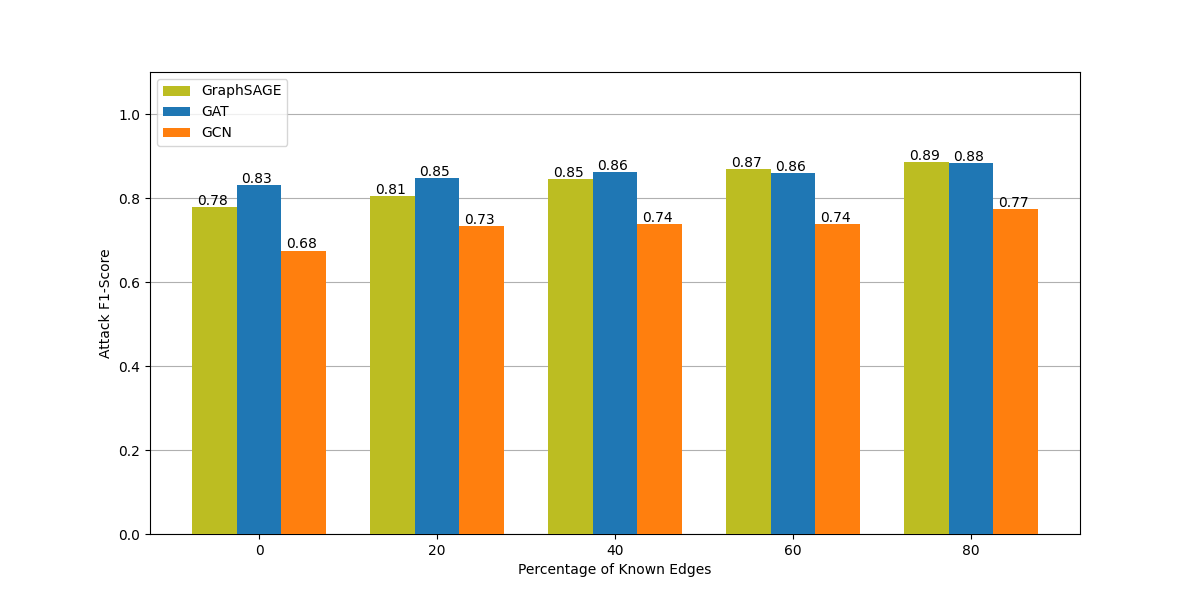
\includegraphics[width=\textwidth]{attack-3-cora-citeseer}
                    \caption{Attack 3 - $D_{f_t} = CiteSeer$ and $D_A = Cora$}
                    \label{figure:eval-att3-cora-citeseer}
                \end{center}
            \end{figure}

            \begin{figure}[h]
                \begin{center}
                    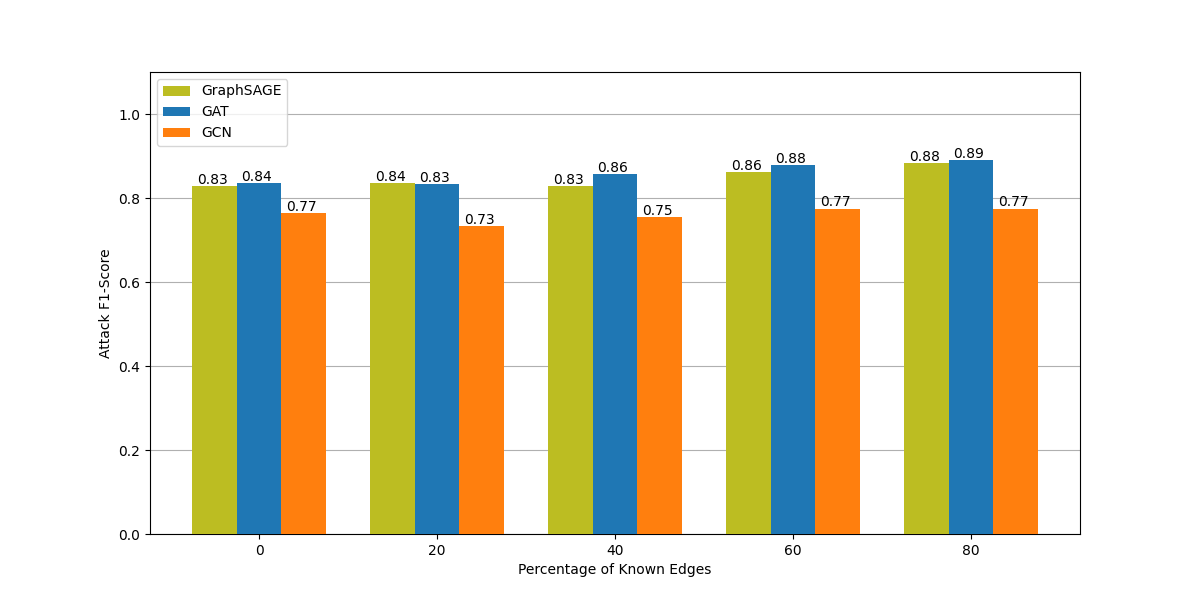
\includegraphics[width=\textwidth]{attack-3-pubmed-citeseer}
                    \caption{Attack 3 - $D_{f_t} = CiteSeer$ and $D_A = Pubmed$}
                    \label{figure:eval-att3-pubmed-citeseer}
                \end{center}
            \end{figure}

            Evaluating \emph{Attack 3}, we note, that the average attack performance of our baseline ($0.7562$ F1-Score) is higher than the average baseline performance of \emph{Attack 1} but lower than the average baseline performance of \emph{Attack 2}.
            The results differ, based on the used datasets $D_{f_t}$ and $D_A$ and the architecture of the target model.
            We achieve a minimum baseline attack performance of $0.6272$ F1-Score with $D_{f_t}$ being the Cora dataset, the attack model being trained on the Pubmed dataset and the target model being a Graph Convolutional Neural Network.
            However, when our target model is a Graph Attention Network, which was trained on the CiteSeer dataset, while the attack model was trained on the Pubmed dataset, we can achieve a maximum baseline attack performance of $0.8297$ F1-Score.  
            Like in the other experiments, the attack performance mostly increases, while the amount of known edges rises.
            This leads to an improvement up to $0.20$ F1-Score.
            With respect to all performed attacks, the average F1-Score is $0.8001$.
            Table \refeq{table:attack3-best-and-worst-performance} presents the F1-Scores of our best and worst attacks.
            
            \vspace{0.48cm}
            \begin{table}[!h]
                \centering
                \footnotesize
                \begin{tabular}{l|l|l|l|l|}
                \toprule
                Target Model & $D_{f_t}$ & $G_A$ Distribution & $\alpha$ & F1-Score \\
                \midrule 
                GAT & CiteSeer & Cora   & 0.8 & $0.8986$ \\
                GCN & Cora     & Pubmed & 0.0 & $0.6272$ \\
                
                \bottomrule
                \end{tabular}
                \caption{Attack-3: Best and Worst Attack Performance}
                \label{table:attack3-best-and-worst-performance}
            \end{table}
        
        The following two tables provide an overview of the best attack performances (Table \refeq{table:attack-best-results-all}) and of the average attack performances on our three target model architectures (Table \refeq{table:attack-avg-results-all}) with respect to all our three attack types.

        \vspace{0.48cm}
        \begin{table}[!h]
            \centering
            \footnotesize
            \begin{tabular}{l|l|l|l|}
                \toprule
                Target Model & Attack 1 & Attack 2 & Attack 3 \\
                \midrule
                GraphSAGE & $0.7577$ & $0.8275$ & $0.8149$ \\
                GAT & $0.8024$ & $0.8923$ & $0.8985$ \\
                GCN & $0.8110$ & $0.8732$ & $0.8777$ \\
                
                \bottomrule
            \end{tabular}
            \caption{Best Attack Performances on Target Models (F1-Score)}
            \label{table:attack-best-results-all}
          \end{table}
        
        \vspace{0.48cm}
        \begin{table}[!h]
            \centering
            \footnotesize
            \begin{tabular}{l|l|l|l|}
                \toprule
                Target Model & Attack 1 & Attack 2 & Attack 3 \\
                \midrule
                GraphSAGE & $0.6943$ & $0.7796$ & $0.7808$ \\
                GAT & $0.7529$ & $0.8251$ & $0.8210$ \\
                GCN & $0.7766$ & $0.8100$ & $0.7985$ \\
                
                \bottomrule
            \end{tabular}
            \caption{Average Attack Performances on Target Models (F1-Score)}
            \label{table:attack-avg-results-all}
        \end{table}
    
    We notice, that sometimes the results of \emph{Attack 3} are more effective than \emph{Attack 2} (Table \refeq{table:attack-best-results-all}), which is against our intuition, since \emph{Attack 3} uses different distribution datasets.
    This phenomenon can be explained with the size of $G_A$.
    In \emph{Attack 2} $G_A$ is much smaller, meaning that less training data can be provided to train the attack model.
    Since $G_A$ is a complete dataset - Cora, CiteSeer or Pubmed - in \emph{Attack 3}, the attack model has more data it can be trained on, leading to a better attack performance.
    In general however (Table \refeq{table:attack-avg-results-all}), we observe that \emph{Attack 2} scores better than \emph{Attack 3} on all target models.

    \section{Possible Defense}
        One possible defense, which already has been presented by He et al. \cite{DBLP:journals/corr/abs-2005-02131}, is to minimize the posterior output vector of $f$. 
        Meaning that instead of providing the complete posterior output of $f$'s prediction, $f$ could only present the top $k$ posteriors.
        In that way the adversary must attack the target model based on less information which makes the attack less effective.
        Since the performed attacks are very similar and only the architecture and functionality of the target model varies, we can assume, that the defense would lead to a similar drop of attack performance in our work.
        
        However, if we assume, that $f$ always provides the complete output posterior, there still exist some methods to mitigate our attacks. 
        Like He et al. proposed in their work, it is also possible to defend against these attacks by leveraging differential privacy (DP) and adversarial examples.
        More specifically we could adopt edge-Differential Privacy \cite{Hay_accurateestimation, lu2020protect, 8345716, Zhang_2015}.
        The approach of Zhang et al. \cite{Zhang_2015} specifies a probability distribution over possible outputs to ensure DP.
        While it is carefully defined to maximize the utility for the given input, it still provides the required privacy level.
        Like shown in previous work \cite{jia2020attriguard, jia2019memguard}, it is also possible to fool the adversary by adding noise to the prediction of the target model.

    \section{Summary of Results}
        To sum up, we made the following observations during our experiments.
        First, our attacks can successfully steal links from inductive trained Graph Neural Networks.
        For example we were able to steal links from Graph Convolutional Networks with F1-Scores up to $0.8955$, which shows the effectiveness of our attacks.
        Second, there exists a dependence between the amount of known edges the adversary has and the attack performance. 
        The more background knowledge the adversary has, the better the results.
        Furthermore, we also achieve good results with our transferring attack.
        However, the performance varies dependent on the shadow dataset.
        But in total the different distribution does not really impact the performance, since the results are similar to same dataset distribution attacks. 
        We observe, that the average attack performance of \emph{Attack 1} scores worst on all our target models.
        We notice an average improvement of $0.09$ F1-Score for GraphSAGE, $0.07$ F1-Score for Graph Attention Networks and $0.03$ F1-Score for Graph Convolutional Networks, when we compare the concatenation of the posteriors (\emph{Attack 1}) with the sampling of features based on the posteriors (\emph{Attack 2 and Attack 3}).
        We lastly note, that our attacks perform worst on the GraphSAGE GNN meaning, that these networks seem to be the most resistant ones.

 % Evaluation

\chapter{Discussion}

    \section{Findings}
        In this thesis we wanted to find out, whether it is possible to efficiently steal links from the training graph of a graph neural network, that has been trained inductively.
        Besides this main question, we also analysed the impact of different distribution datasets on the performance of our attacks and how the choice of features, used to train the attack model, can increase the accuracy of the adversary.

        We found that an adversary with black box access to an inductive trained graph neural network is able to efficiently steal links from the target models training graph.
        To achieve this, the adversary has multiple strategies which differ in the choice of features used to train the attack model and in the dataset distribution of the shadow dataset.
        We saw, that the attack performance is better, when we sample features on the posterior outputs of the target model instead of using them directly.
        We therefor compared the concatenation of the posteriors and a distance vector containing values of eight different distance metrics, that measure the similarity between the posteriors, being the input for our attack model.
        Furthermore we found, that the attack performance is similar when using different dataset distributions to train our attack model.
        More precisely, we are able to steal links using a transferring attack almost as accurate as using a shadow dataset from the same distribution like the one, the target model was trained on.
        Therefor we compared the performance of attack models that have been trained on one of our three datasets Cora, CiteSeer or Pubmed while the target model was trained on another dataset, that differs the one the attacker used.

    \section{Impact}
        Since training data for machine learning models can often be deemed confidential, we note, that stealing links from the training graph of an inductive trained graph neural network leads to a huge privacy risk.
        The data owner often spends lots of time and resources preprocessing the data and thus can claim the dataset as intellectual property.
        Furthermore, the training data of a graph neural network often contains sensitive data, that can be revealed using our attacks.
        This can include health data of patients or sensitive social relationships of social network users.
        Since graphs and therefor graph neural networks are getting more popular every day, our attacks have a huge impact on the privacy of training data.
        Furthermore, it seems to be hard to protect against our attacks without a tradeoff between good privacy and functionality of the target model. 

    \section{Future Work}
        In future work it would be interesting to see how link stealing attacks perform on target models, that have been trained to perform different downstream tasks.
        Since all of our target models are trained to perform node classification, it would be interesting to see, whether the task of the graph neural network has some impact on the attack accuracy.
        Furthermore, one could spend some time figuring out, whether there is a better way of using the raw posteriors as input for the attack model.
        Since we only concatenate them to one big vector, maybe there is a better way of using them, which leads to better results.
        Also one could search for even better feature samples than eight distance metrics to use as input for the attack model.
        Last but definitely not least, one could search for good defenses against our attacks.
        Since revealing links from the train graph brings huge privacy risks, finding an efficient defense against our attack may be the most important future work. % Discussion

\chapter{Conclusion}
    Since machine learning and big data are huge points of interest for many people and companies, the need for privacy preserving approaches is indispensable.
    With our work we want to contribute, by showing privacy risks in common used training processes.
    That's why we propose link stealing attacks on inductive trained graph neural networks.
    Using our attacks, we are able to successfully steal links from a graph that was used to inductively train the target graph neural network model.
    Only with black box access to the target model an adversary is able to reveal sensitive information about that graph leading to huge privacy concerns.
    We investigated the performance of our attacks using three types of graph neural networks - GraphSAGE, Graph Attention Networks and Graph Convolutional Networks and trained them on three common used graph datasets - Cora, CiteSeer and Pubmed - to perform node classification.
    In our experiments we also considered different inputs for our attack model.
    For some experiments, we concatenate the posterior outputs of our target model, for some others, we sample new features based on the similarity of the posteriors using eight different distance metrics.   
    We showed, that we are able to efficiently predict whether any two nodes in the training graph are linked or not only considering black box access and some shadow dataset.
    We also showed, that transferring attacks perform with similar results while being trained on different dataset distributions.

    To conclude this thesis, we saw that a common used training procedure can lead to significant privacy risks, since the target graph neural network model can be used to reveal sensitive information about the graph that was used for training.
    We saw that only black box access and some shadow dataset is enough to perform our attacks and that the performance increases with rising background knowledge.
 % Conclusion

%% ----------------------------------------------------------------
% Now begin the Appendices, including them as separate files

\addtocontents{toc}{\vspace{2em}} % Add a gap in the Contents, for aesthetics

%% ----------------------------------------------------------------
%\lhead{\emph{List of Figures}}  % Set the left side page header to "List if Figures"
\listoffigures  % Write out the List of Figures

%% ----------------------------------------------------------------
%\lhead{\emph{List of Tables}}  % Set the left side page header to "List of Tables"
\listoftables  % Write out the List of Tables

% \appendix % Cue to tell LaTeX that the following 'chapters' are Appendices

% Appendix A
\chapter*{Appendix}
    \begin{table}[h]
        \centering
        \footnotesize
        \begin{tabular}{l|c}
        \toprule
        Metrics & Definition \\
        \midrule
        Cosine & $1 - \dfrac{f_t(u)\cdot f_t(v)}{\left||f_t(u)\right||_2\left||f_t(v)\right||_2}$ \\
        Euclidean & $\left||f_t(u) - f_t(v)\right||_2$ \\
        Correlation & $1-\dfrac{(f_t(u)-\overline{f_t(u)}) \cdot(f_t(v)-\overline{f_t(v)})}{||(f_t(u)-\overline{f_t(u)})||_{2}||(f_t(v)-\overline{f_t(v)})||_{2}}$ \\
        Chebyshev & $\max _{i}\left|f_{t_i}(u)-f_{t_i}(v)\right|$ \\
        Braycurtis & $\dfrac{\sum\left|f_{t_i}(u)-f_{t_i}(v)\right|} {\sum\left|f_{t_i}(u)+f_{t_i}(v)\right|}$ \\
        Manhattan & $\sum{i}\left|f_{t_i}(u)-f_{t_i}(v)\right|$ \\
        Canberra & $\sum_{i} \dfrac{\left|f_{t_i}(u)-f_{t_i}(v)\right|}{\left|f_{t_i}(u)\right|+\left|f_{t_i}(v)\right|}$ \\
        Sqeuclidean & $\left||f_t(u) - f_t(v)\right||_2^2$ \\
        \bottomrule
        \end{tabular}
        \caption{Distance metrics: $f_{t_i}(u)$ represents the $i$-th component of $f_t(u)$.}
        \label{table:distance}
    \end{table}

    \vspace{1cm}
    \begin{table}[!h]
        \centering
        \footnotesize
        \begin{tabular}{l|l|}
          \toprule
          Notation & Description \\
          \midrule
          $f_t$ & Target GNN Model \\
          $D_{f_t}$ & Data set used to train $f_t$ \\
          $A$ & Adversary \\
          $D_A$ & Data set used to train $A$ \\
          $G_A$ & Graph used to sample $D_A$ \\
          $\alpha$ & Percentage of known edges in $G_A$ \\
          $G_A^{0.4}$ & Graph used to sample $D_A$ with 40\% known edges \\
          $f_A$ & Shadow GNN Model, that is involved in training $A$ \\
          $D_{f_A}$ & Data set used to train $f_A$ \\
          $G_s$ & Incomplete Graph, $A$ performs link stealing attacks on \\
          \bottomrule
        \end{tabular}
        \caption{Notations}
        \label{table:notations}
      \end{table}

    \begin{figure}[h]
      \begin{center}
        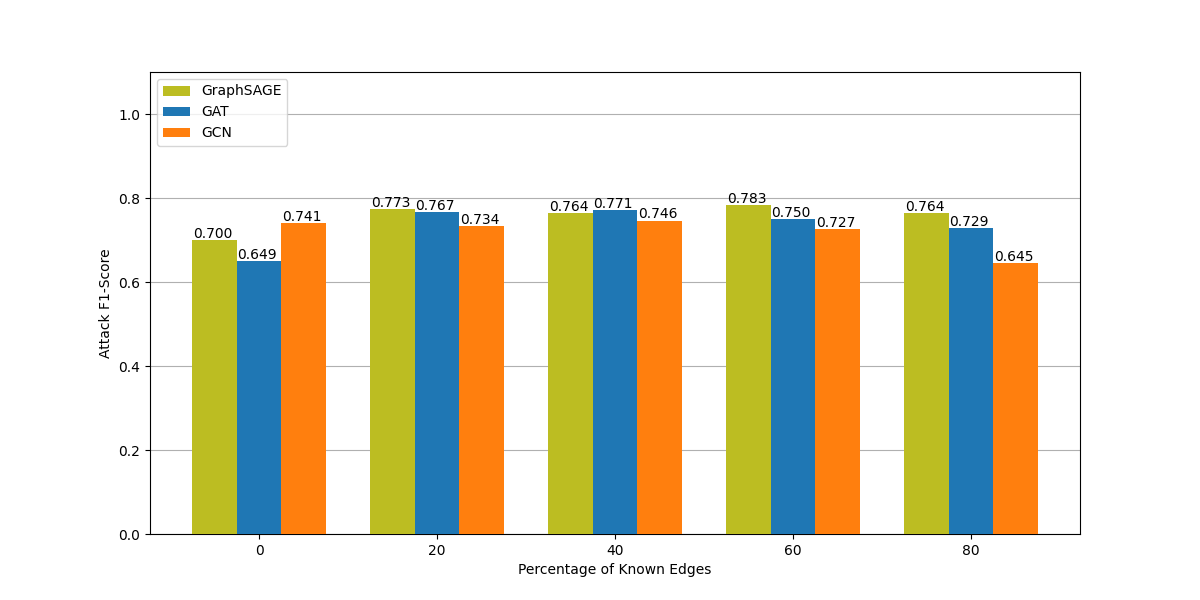
\includegraphics[width=\textwidth]{attack-1-cora}
        \caption[Attack 1 - $D_{f_t} = Cora$]{Performance of \emph{Attack 1} in F1-Score (y-axis) on our three GNN architectures with rising amount of known edges (x-axis). The target model $f_t$ was trained on the Cora data set.}
        \label{figure:eval-att1-cora}
      \end{center}
    \end{figure}

    \begin{figure}[h]
      \begin{center}
        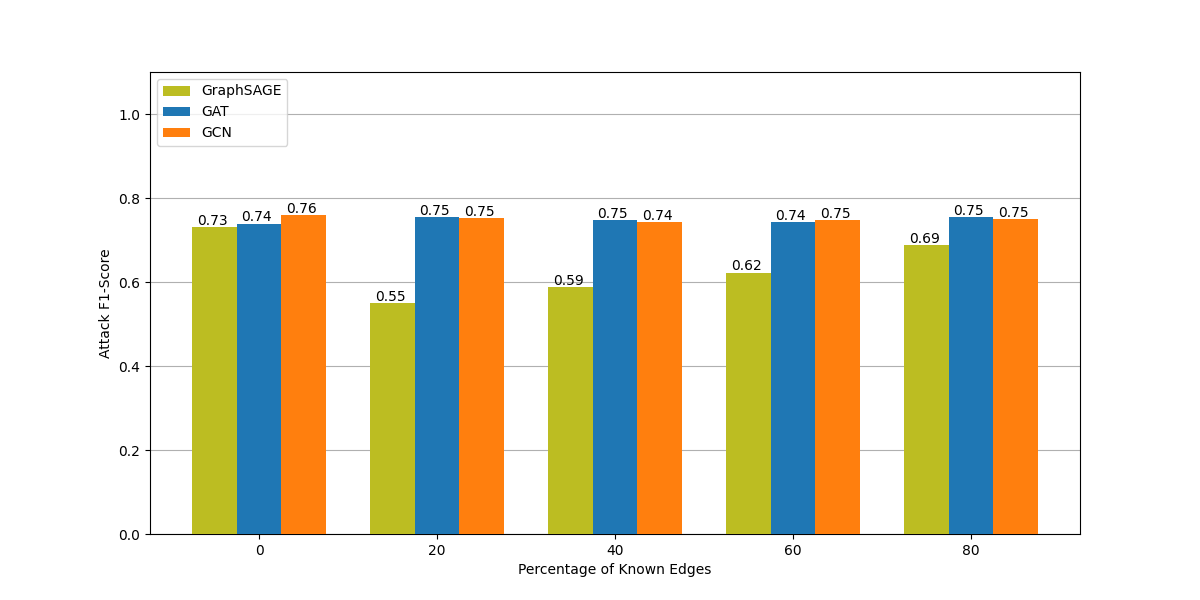
\includegraphics[width=\textwidth]{attack-1-pubmed}
        \caption[Attack 1 - $D_{f_t} = Pubmed$]{Performance of \emph{Attack 1} in F1-Score (y-axis) on our three GNN architectures with rising amount of known edges (x-axis). The target model $f_t$ was trained on the Pubmed data set.}
        \label{figure:eval-att1-pubmed}
      \end{center}
    \end{figure}

    \begin{figure}[h]
      \begin{center}
          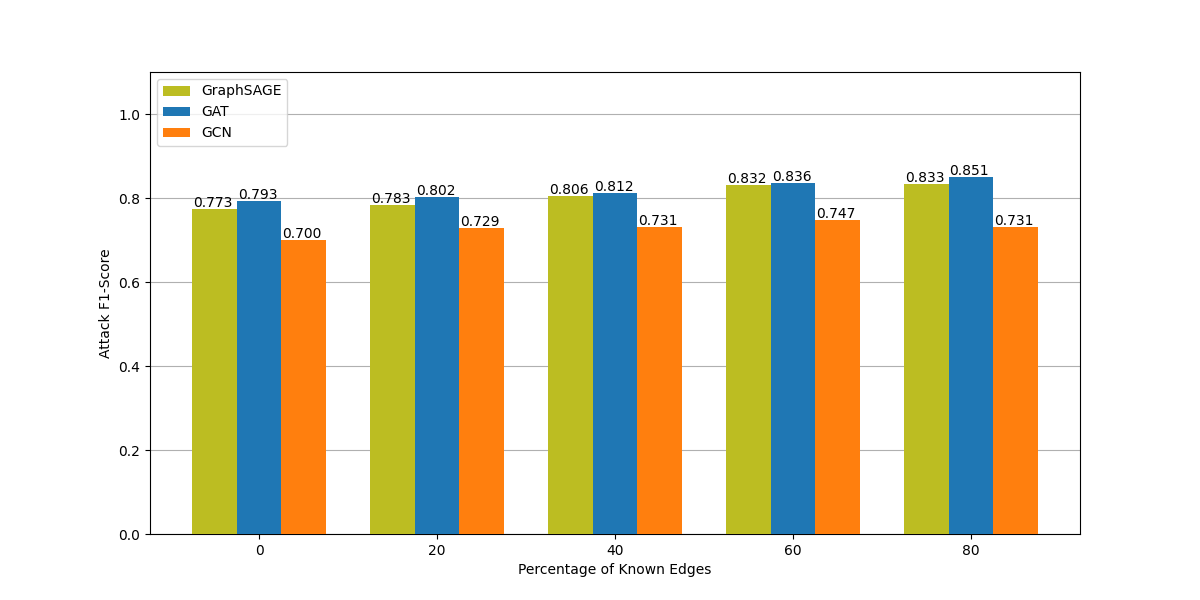
\includegraphics[width=\textwidth]{attack-2-cora}
          \caption[Attack 2 - $D_{f_t} = Cora$]{Performance of \emph{Attack 2} in F1-Score (y-axis) on our three GNN architectures with rising amount of known edges (x-axis). The target model $f_t$ was trained on the Cora data set.}
          \label{figure:eval-att2-cora}
      \end{center}
    \end{figure}

    \begin{figure}[h]
      \begin{center}
          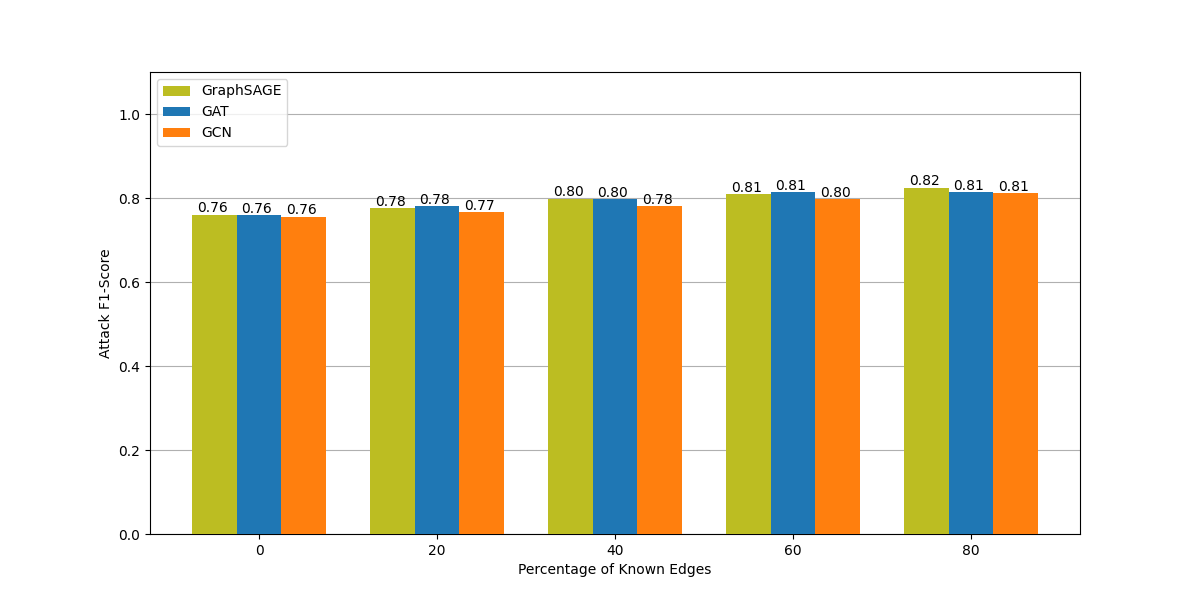
\includegraphics[width=\textwidth]{attack-2-pubmed}
          \caption[Attack 2 - $D_{f_t} = Pubmed$]{Performance of \emph{Attack 2} in F1-Score (y-axis) on our three GNN architectures with rising amount of known edges (x-axis). The target model $f_t$ was trained on the Pubmed data set.}
          \label{figure:eval-att2-pubmed}
      \end{center}
    \end{figure}

    \begin{figure}[h]
      \begin{center}
          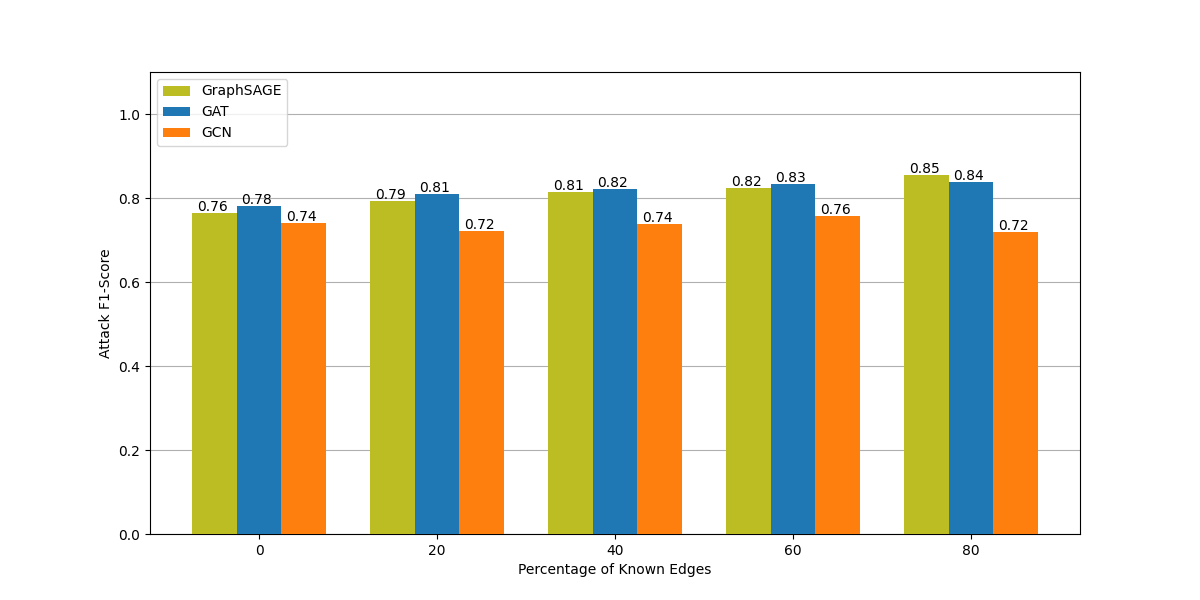
\includegraphics[width=\textwidth]{attack-3-citeseer-cora}
          \caption[Attack 3 - $D_{f_t} = Cora$ and $D_A = CiteSeer$]{Performance of \emph{Attack 3} in F1-Score (y-axis) on our three GNN architectures with rising amount of known edges (x-axis). The target model $f_t$ was trained on the Cora data set while the shadow model $f_A$ was trained on the CiteSeer data set.}
          \label{figure:eval-att3-citeseer-cora}
      \end{center}
  \end{figure}

  \begin{figure}[h]
      \begin{center}
          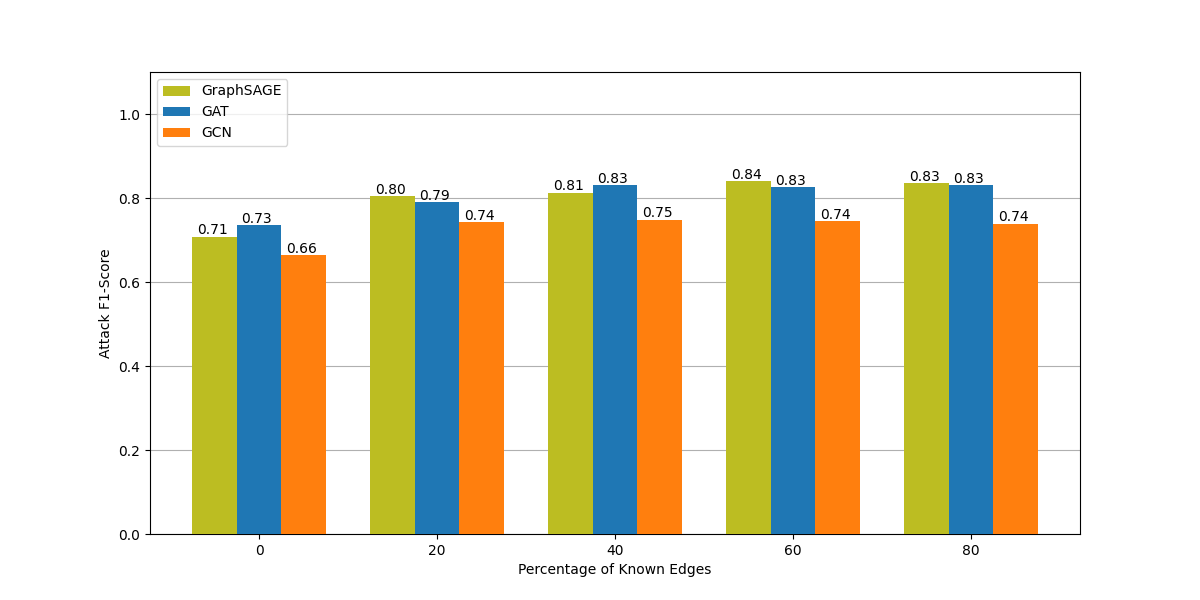
\includegraphics[width=\textwidth]{attack-3-pubmed-cora}
          \caption[Attack 3 - $D_{f_t} = Cora$ and $D_A = Pubmed$]{Performance of \emph{Attack 3} in F1-Score (y-axis) on our three GNN architectures with rising amount of known edges (x-axis). The target model $f_t$ was trained on the Cora data set while the shadow model $f_A$ was trained on the Pubmed data set.}
          \label{figure:eval-att3-pubmed-cora}
      \end{center}
  \end{figure}

  \begin{figure}[h]
    \begin{center}
        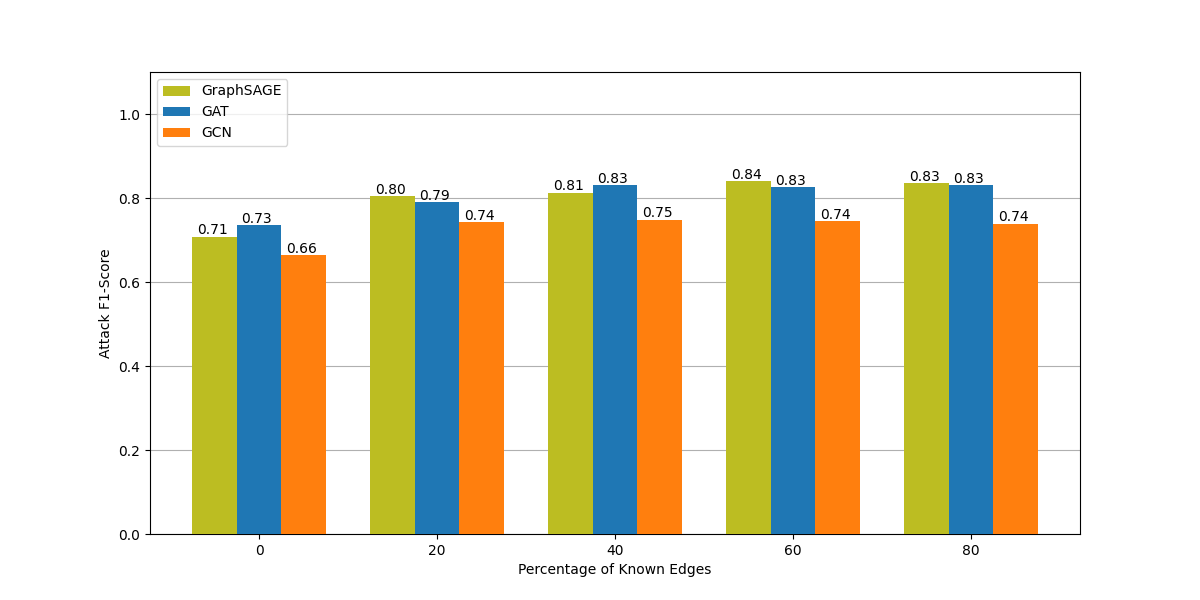
\includegraphics[width=\textwidth]{attack-3-pubmed-cora}
        \caption[Attack 3 - $D_{f_t} = Pubmed$ and $D_A = Cora$]{Performance of \emph{Attack 3} in F1-Score (y-axis) on our three GNN architectures with rising amount of known edges (x-axis). The target model $f_t$ was trained on the Pubmed data set while the shadow model $f_A$ was trained on the Cora data set.}
        \label{figure:eval-att3-cora-pubmed}
    \end{center}
  \end{figure}

  \begin{figure}[h]
      \begin{center}
          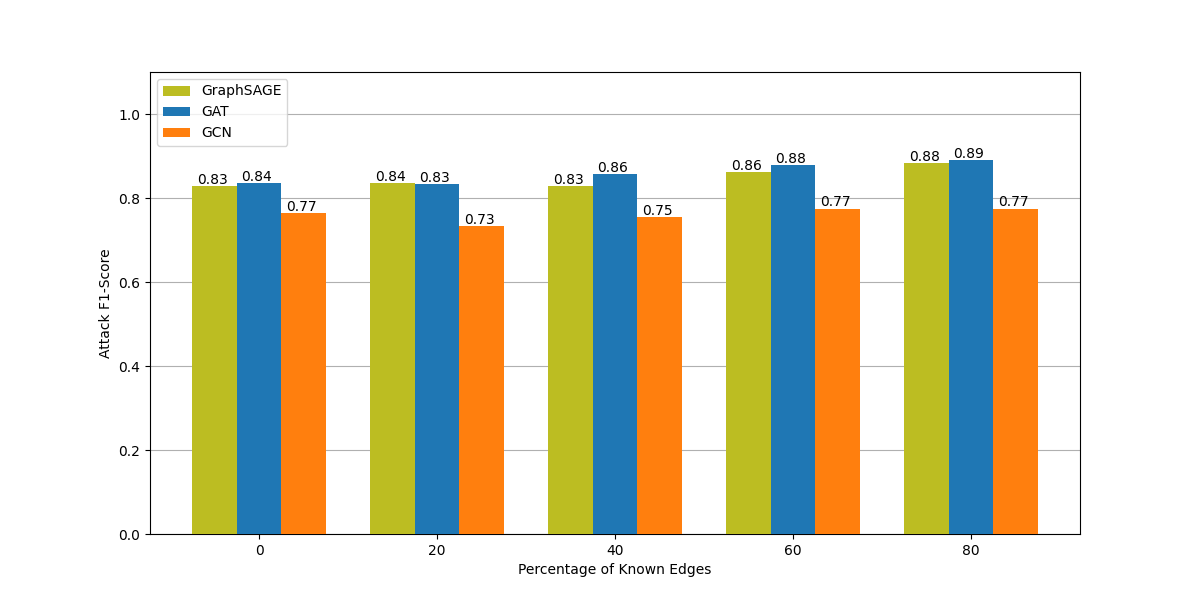
\includegraphics[width=\textwidth]{attack-3-pubmed-citeseer}
          \caption[Attack 3 - $D_{f_t} = Pubmed$ and $D_A = CiteSeer$]{Performance of \emph{Attack 3} in F1-Score (y-axis) on our three GNN architectures with rising amount of known edges (x-axis). The target model $f_t$ was trained on the Pubmed data set while the shadow model $f_A$ was trained on the CiteSeer data set.}
          \label{figure:eval-att3-citeseer-pubmed}
      \end{center}
  \end{figure} % tables

\addtocontents{toc}{\vspace{2em}}  % Add a gap in the Contents, for aesthetics
\backmatter

%% ----------------------------------------------------------------
\label{Bibliography}
%\nocite{*}
%\lhead{\emph{Bibliography}}  % Change the left side page header to "Bibliography"
%\  % Use the "unsrtnat" BibTeX style for formatting the Bibliography
%\bibliographystyle{unsrtdin}
\bibliographystyle{IEEEtran}
\bibliography{src/Bibliography}  % The references (bibliography) information are stored in the file named "Bibliography.bib"

\end{document}  % The End
%% ----------------------------------------------------------------
